\documentclass[10pt,landscape]{article}
\usepackage{multicol}
\usepackage{calc}
\usepackage{ifthen}
\usepackage[landscape]{geometry}
\usepackage{graphicx}
\usepackage{amsmath, amssymb, amsthm}
\usepackage{latexsym, marvosym}
\usepackage{pifont}
\usepackage{lscape}
\usepackage{float}
\usepackage{graphicx}
\usepackage{array}
\usepackage{booktabs}
\usepackage[bottom]{footmisc}
\usepackage{xcolor}
	\definecolor{GTBlue}{RGB}{0, 48, 87}
	\definecolor{GTGold}{RGB}{234, 170, 0}
	\definecolor{GTLBlue}{RGB}{24, 121, 219}
	\definecolor{FSGarnet}{RGB}{120, 47, 64}
	\definecolor{FSLGarnet}{RGB}{165, 14, 50}
	\definecolor{FSGold}{RGB}{206, 184, 136}
\usepackage{tikz}
\usetikzlibrary{shapes}
\usepackage{pdfpages}
\usepackage{wrapfig}
\usepackage{enumitem}
\setlist[description]{leftmargin=0pt}
\usepackage{xfrac}
\usepackage[nice]{nicefrac}
\usepackage{multirow}
\usepackage{vwcol}
\usepackage[pdftex,
            pdfauthor={Oscar Martinez},
            pdftitle={Probability Cheatsheet},
            pdfsubject={I used William Chen's Fantastic Probability Cheat Sheet and modified it for my needs for FSU's Econ PhD Econometrics I.},
            pdfkeywords={probability} {statistics} {cheatsheet} {pdf} {cheat} {sheet} {formulas} {equations}
            ]{hyperref}
\usepackage[
            open,
            openlevel=2
            ]{bookmark}
\usepackage{relsize}
\usepackage{rotating}

 \newcommand\independent{\protect\mathpalette{\protect\independenT}{\perp}}
    \def\independenT#1#2{\mathrel{\setbox0\hbox{$#1#2$}%
    \copy0\kern-\wd0\mkern4mu\box0}} 
            
\newcommand{\noin}{\noindent}    
\newcommand{\logit}{\textrm{logit}} 
\newcommand{\var}{\textrm{Var}}
\newcommand{\cov}{\textrm{Cov}} 
\newcommand{\corr}{\textrm{Corr}} 
\newcommand{\N}{\mathcal{N}}
\newcommand{\Bern}{\textrm{Bern}}
\newcommand{\Bin}{\textrm{Bin}}
\newcommand{\Beta}{\textrm{Beta}}
\newcommand{\Gam}{\textrm{Gamma}}
\newcommand{\Expo}{\textrm{Expo}}
\newcommand{\Pois}{\textrm{Pois}}
\newcommand{\Unif}{\textrm{Unif}}
\newcommand{\Geom}{\textrm{Geom}}
\newcommand{\NBin}{\textrm{NBin}}
\newcommand{\Hypergeometric}{\textrm{HGeom}}
\newcommand{\HGeom}{\textrm{HGeom}}
\newcommand{\Mult}{\textrm{Mult}}
\newcommand{\RA}{\Rightarrow}
\renewcommand{\to}{\rightarrow}
\newcommand{\Reals}{\mathbb{R}}

\newcolumntype{H}{>{\setbox0=\hbox\bgroup}c<{\egroup}@{}}
\newcolumntype{Z}{>{\setbox0=\hbox\bgroup}c<{\egroup}@{\hspace*{-\tabcolsep}}}

\geometry{top=.4in,left=.2in,right=.2in,bottom=.4in}

\pagestyle{empty}
\makeatletter
\renewcommand{\section}{\@startsection{section}{1}{0mm}%
                                {-1ex plus -.5ex minus -.2ex}%
                                {0.5ex plus .2ex}%x
                                {\normalfont\large\bfseries}}
\renewcommand{\subsection}{\@startsection{subsection}{2}{0mm}%
                                {-1explus -.5ex minus -.2ex}%
                                {0.5ex plus .2ex}%
                                {\normalfont\normalsize\bfseries}}
\renewcommand{\subsubsection}{\@startsection{subsubsection}{3}{0mm}%
                                {-1ex plus -.5ex minus -.2ex}%
                                {1ex plus .2ex}%
                                {\normalfont\small\bfseries}}
\makeatother

\setcounter{secnumdepth}{0}

\setlength{\parindent}{0pt}
\setlength{\parskip}{0pt plus 0.5ex}

% -----------------------------------------------------------------------

\usepackage{titlesec}

\titleformat{\section}
{\color{FSLGarnet}\normalfont\large\bfseries}
{\color{FSLGarnet}\thesection}{1em}{}
\titleformat{\subsection}
{\color{FSGold}\normalfont\normalsize\bfseries}
{\color{FSGold}\thesection}{1em}{}
% Comment out the above 5 lines for black and white

\DeclareMathOperator*{\SumInt}{%
	\mathchoice%
	{\ooalign{$\displaystyle\sum$\cr\hidewidth$\displaystyle\int$\hidewidth\cr}}
	{\ooalign{\raisebox{.14\height}{\scalebox{.7}{$\textstyle\sum$}}\cr\hidewidth$\textstyle\int$\hidewidth\cr}}
	{\ooalign{\raisebox{.2\height}{\scalebox{.6}{$\scriptstyle\sum$}}\cr$\scriptstyle\int$\cr}}
	{\ooalign{\raisebox{.2\height}{\scalebox{.6}{$\scriptstyle\sum$}}\cr$\scriptstyle\int$\cr}}
}

\titlespacing{\subsection}{0pt}{*0}{*0}

\begin{document}

\raggedright
\footnotesize
\begin{multicols*}{3}

% multicol parameters
% These lengths are set only within the two main columns
%\setlength{\columnseprule}{0.25pt}
\setlength{\premulticols}{1pt}
\setlength{\postmulticols}{1pt}
\setlength{\multicolsep}{1pt}
\setlength{\columnsep}{2pt}
\setlength{\abovedisplayskip}{2pt}
\setlength{\belowdisplayskip}{2pt}




%%%%%%%%%%%%%%%%%%%%%%%%%%%%%%%%%%%%
%%% TITLE
%%%%%%%%%%%%%%%%%%%%%%%%%%%%%%%%%%%%

%\begin{center}
%    {\color{blue} \Large{\textbf{Probability Cheatsheet v2.0}}} \\
%   % {\Large{\textbf{Probability Cheatsheet}}} \\
%    % comment out line with \color{blue} and uncomment above line for b&w
%\end{center}

%%%%%%%%%%%%%%%%%%%%%%%%%%%%%%%%%%%%
%%% ATTRIBUTIONS
%%%%%%%%%%%%%%%%%%%%%%%%%%%%%%%%%%%%

%\scriptsize

%Compiled by William Chen (\url{http://wzchen.com}) and Joe Blitzstein, with contributions from Sebastian Chiu, Yuan Jiang, Yuqi Hou, and Jessy Hwang. Material based on Joe Blitzstein's (\texttt{\href{http://twitter.com/stat110}{@stat110}}) lectures (\url{http://stat110.net}) and Blitzstein/Hwang's Introduction to Probability textbook (\url{http://bit.ly/introprobability}). Licensed under \texttt{\href{http://creativecommons.org/licenses/by-nc-sa/4.0/}{CC BY-NC-SA 4.0}}. Please share comments, suggestions, and errors at \url{http://github.com/wzchen/probability_cheatsheet}.
%
%\begin{center}
%    Last Updated \today
%\end{center}

% Cheatsheet format from
% http://www.stdout.org/$\sim$winston/latex/

%%%%%%%%%%%%%%%%%%%%%%%%%%%%%%%%%%%%
%%% BEGIN CHEATSHEET
%%%%%%%%%%%%%%%%%%%%%%%%%%%%%%%%%%%%

\section{Introduction} \hrule height 2pt 
\scriptsize
This is a cheatsheet compiled for the First-Year Econometrics sequence at Florida State University as taught by Dr. Zuehlke. While a lot of the material presented here was compiled and aggregated by myself (but not invented!), I could not have done this without the original template as graciously provided by William Chen. His website is \url{http://wzchen.com}, and he provides the original ``Probability Cheatsheet" there. His version is far more expansive (and arguably better) than mine. Additional thanks are also due to Dr. Zuehlke whose lecture notes compose a large extent of this cheatsheet. The goal of this cheatsheet is to provide a quick refresher or desktop reference for the forgetful econometrician. Any errors are my own and please don't hesitate to contact me with suggestions or corrections at \url{oam18@my.fsu.edu} .

\hrule height 2pt
\section{\huge Probability Concepts}
\hrule height 2pt

\section{Counting}\hrule height 2pt 

% \subsection{Set Theory}
%
% \begin{description}
%     \item[Sets and Subsets] - A set is a collection of distinct objects. $A$ is a subset of $B$ if every element of $A$ is also included in $B$.
%     \item[Empty Set] - The empty set, denoted $\emptyset$, is the set that contains nothing.
%     \item[Set Notation] - Note that ${\bf {\bf A}} \cup {\bf B}$, ${\bf A} \cap {\bf B}$, and ${\bf A^c}$ are all sets too.
%     \begin{description}
%         \item[Union] - ${\bf A} \cup {\bf B}$ (read \emph{{\bf A} union {\bf B}}) means ${\bf A}\ or\ {\bf B}$
%         \item[Intersection] - ${\bf A} \cap {\bf B}$ (read \emph{{\bf A} intersect {\bf B}}) means ${\bf A}\ and \ {\bf B}$
%         \item[Complement] - ${\bf A^c}$ (read \emph{{\bf A} complement}) occurs whenever ${\bf A}$ does not occur
%     \end{description}
%     \item[Disjoint Sets] - Two sets are disjoint if their intersection is the empty set (e.g. they don't overlap).
%     \item[Partition] - A set of subsets ${\bf A}_1, {\bf A}_2, {\bf A}_3, ... {\bf A}_n$ partition a space if they are disjoint and cover all possible outcomes (e.g. their union is the entire set). A simple case of a partitioning set of subsets is ${\bf A}, {\bf A^c}$
%         \item[Principle of Inclusion-Exclusion] - Helps you find the probabilities of unions of events. 
%         \[ P ({\bf A} \cup {\bf B}) = P({\bf A}) + P({\bf B}) - P({\bf A} \cap {\bf B}) \]
%         \[P(\textnormal{Union of many events}) = \textnormal{Singles} - \textnormal{Doubles} + \textnormal{Triples} - \textnormal{Quadruples} \dots\]
%
%
% \end{description}
    \subsection{Addition \& Multiplication Rules} 
    \begin{minipage}{\linewidth}
            \centering
            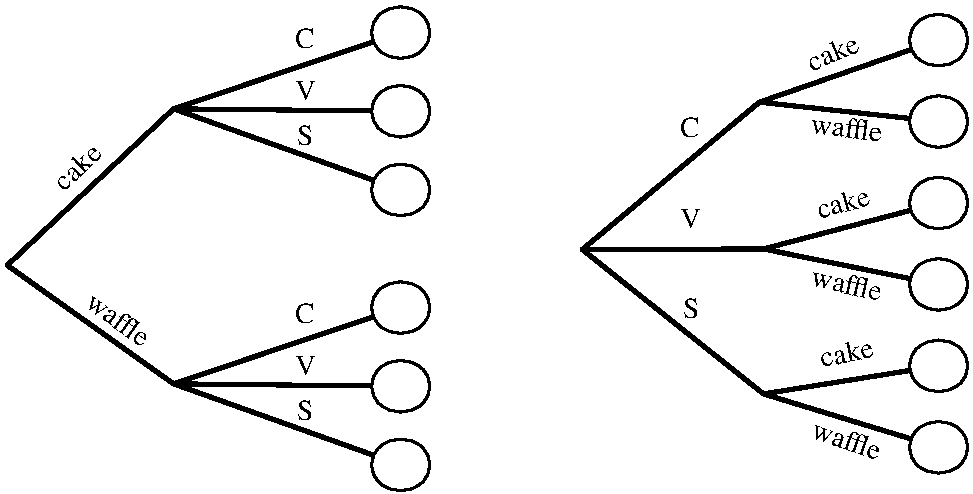
\includegraphics[width=2in]{figures/icecream.pdf}
        \end{minipage}
        
 Let's say we have a compound experiment (an experiment with multiple components). If the 1st component has $n_1$ possible outcomes, the 2nd component has $n_2$ possible outcomes, \dots, and the $r$th component has $n_r$ possible outcomes. If only one component can be chosen, then we have $n_1+n_2+ \dots+ n_r$ ways to select an outcome. If you can select one outcome per component, then overall there are $n_1n_2 \dots n_r$ possibilities for the whole experiment.
 
\subsection{Sampling Table}
%   \begin{minipage}{\linewidth}
%            \centering
%             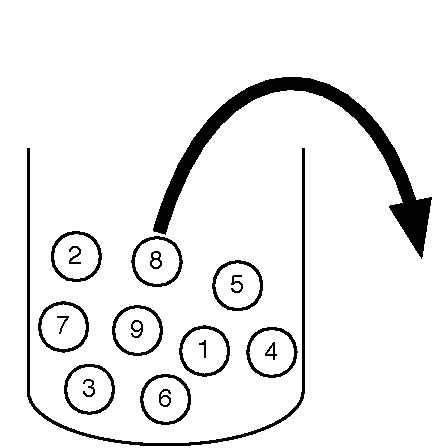
\includegraphics[width=1.2in]{figures/jar.pdf}
%        \end{minipage}
      %  \begin{center}
    The sampling table gives the number of possible samples of size $k$ out of a population of size $n$, under various assumptions about how the sample is collected. 
        %\begin{table}[H]
        \begin{center}
                \setlength{\extrarowheight}{7pt}
            \begin{tabular}{r|cc}
                 & \textbf{Order Matters} & \textbf{Not Matter} \\ \hline
                \textbf{With Replacement} & $\displaystyle n^k$ & $\displaystyle{n+k-1 \choose k}$ \\
                \textbf{Without Replacement} & $\displaystyle\frac{n!}{(n - k)!}$ & $\displaystyle{n \choose k}$
            \end{tabular}
        	
        \end{center}
    
        %\end{table}
    % \item[Experiments/Outcomes] - An experiment generates an outcome from a pre-determined list. For example, a dice roll generates outcomes in the set $\{1, 2, 3, 4, 5, 6\}$
    % \item[Sample Space] - The sample space, denoted $\Omega$, is the set of possible outcomes. Note that the probability of this event is 1, since something in the sample space will always occur.
    % \item[Event] - An event is a subset of the sample space, or a collection of possible outcomes of an experiment. We say that the event has occurred if any of the outcomes in the event have happened.
   
   \subsection{Some Distributions for Discrete Draws}
   \begin{center}
   	\begin{tabular}{ccc}
   		~ & \textbf{Replace} & \textbf{No Replace}  \\
   		\midrule
   		\textbf{Fixed \# trials ($n$)} & Binomial & HGeom \\ 
   		~ & (Bern if $n = 1$) & ~ \\ 
   		\textbf{Draw until $r$ success} & NBin & NHGeom \\ 
   		~ & (Geom if $r = 1$) & ~\\ \bottomrule
   	\end{tabular}
   \end{center}
   
    \subsection{Naive Definition of Probability}  {If all outcomes are equally likely}, the probability of an event $A$ happening is:
        \[P_{\textrm{naive}}(A) = \frac{\textnormal{number of outcomes favorable to $A$}}{\textnormal{number of outcomes}}\]

\section{Thinking Conditionally} \hrule height 2pt 

% \subsection{Set Theory and Statistics}
% %To understand probability it helps to understand basic set theory. An \emph{event} is a set in that it is a collection of possible outcomes of an experiment (or a subset of the sample space). With set theory we can talk about things like unions, intersections, or complements of events.

% \begin{description}
%     \item[Experiments/Outcomes] - An experiment generates an outcome from a pre-determined list. For example, a dice roll generates outcomes in the set $\{1, 2, 3, 4, 5, 6\}$
%     \item[Sample Space] - The sample space, denoted $\Omega$, is the set of possible outcomes. Note that the probability of this event is 1, since something in the sample space will always occur.
%     \item[Event] - An event is a subset of the sample space, or a collection of possible outcomes of an experiment. We say that the event has occurred if any of the outcomes in the event have happened.
% \end{description}

%\subsection{Disjointness Versus Independence}
\subsection{Independence}

    \begin{description}
        % \item[Disjoint Events] - ${\bf A}$ and ${\bf B}$ are disjoint when they cannot happen simultaneously, or
        %   \begin{align*}
        %     P({\bf A} \cap {\bf B}) &= 0\\
        %     {\bf A} \cap {\bf B} &= \emptyset
        %   \end{align*}
        \item[Independent Events] $A$ and $B$ are independent if knowing whether $A$ occurred gives no information about whether $B$ occurred. More formally, $A$ and $B$ (which have nonzero probability) are independent if and only if one of the following equivalent statements holds: 
           \begin{align*} 
            P({A}\cap { B}) &= P({A})P({B}) \\
            P({ A}|{ B}) &= P({A})\\
            P(B|A) &= P(B)
           \end{align*}
        \item[Conditional Independence]  ${A}$ and ${B}$ are conditionally independent given ${C}$ if $P({A}\cap {B}|{C}) = P({A}|{C})P({B}|{C})$. Conditional independence does not imply independence, and independence does not imply conditional independence.
    \end{description}
    
\subsection{Unions, Intersections, and Complements}

    \begin{description}

        \item[De Morgan's Laws] A useful identity that can make calculating probabilities of unions easier by relating them to intersections, and vice versa. Analogous results hold with more than two sets.
           \begin{align*} 
        ({A} \cup { B})^c = {A^c} \cap { B^c} \\
        ({A} \cap {B})^c = { A^c} \cup { B^c}
           \end{align*} 
                  
        % \item[Complements] - The following are true.
        %    \begin{align*} 
        %      {\bf A} \cup {\bf A}^c &= \Omega \\
        %      {\bf A} \cap {\bf A}^c &= \emptyset\\
        %      P({\bf A}) &= 1 -  P({\bf A}^c)
        %    \end{align*} 

    \end{description}

\subsection{Joint, Marginal, and Conditional}

    \begin{description}
        \item[Joint Probability] $P({A} \cap {B}) $ or $P({ A}, {B})$ $ \leftarrow $ Probability of ${ A}$ and ${B}$.
        \item[Marginal (Unconditional) Probability] $P({A})$ $ \leftarrow $ Probability of ${A}$.
        \item[Conditional Probability]  $P({A}|{B}) = P(A,B)/P(B)$ $ \leftarrow $ Probability of ${A}$, given that ${B}$ occurred.
        \item[Conditional Probability \emph{is} Probability]  $P({A}|{ B})$ is a probability function for any fixed $B$. Any theorem that holds for probability also holds for conditional probability.
    %     \item[Bayes' Rule] - Bayes' Rule unites marginal, joint, and conditional probabilities. We use this as the definition of conditional probability.
    % \[P({\bf A}|{\bf B}) = \frac{P({\bf A} \cap {\bf B})}{P({\bf B})} = \frac{P({\bf B}|{\bf A})P({\bf A})}{P({\bf B})}\]
    \end{description}

\subsection{Probability of an Intersection or Union}
\textbf{Intersections via Conditioning}
\begin{align*} 
    P(A\cap B) &= P(A)P(B|A) \\
   P(A\cap B\cap C) &= P(A)P(B|A)P(C|A\cap B) 
   \end{align*}
   \textbf{Unions via Inclusion-Exclusion}
   \begin{align*} 
    P(A \cup B) &= P(A) + P(B) - P(A \cap B) \\
  P(A \cup B \cup C) &= P(A) + P(B) + P(C) - P(A \cap B) \\ 
  & \quad- P(A \cap C) - P(B \cap C)  + P(A \cap B \cap C).
   \end{align*}


%\subsection{Simpson's Paradox}
%\begin{minipage}{\linewidth}
%            \centering
%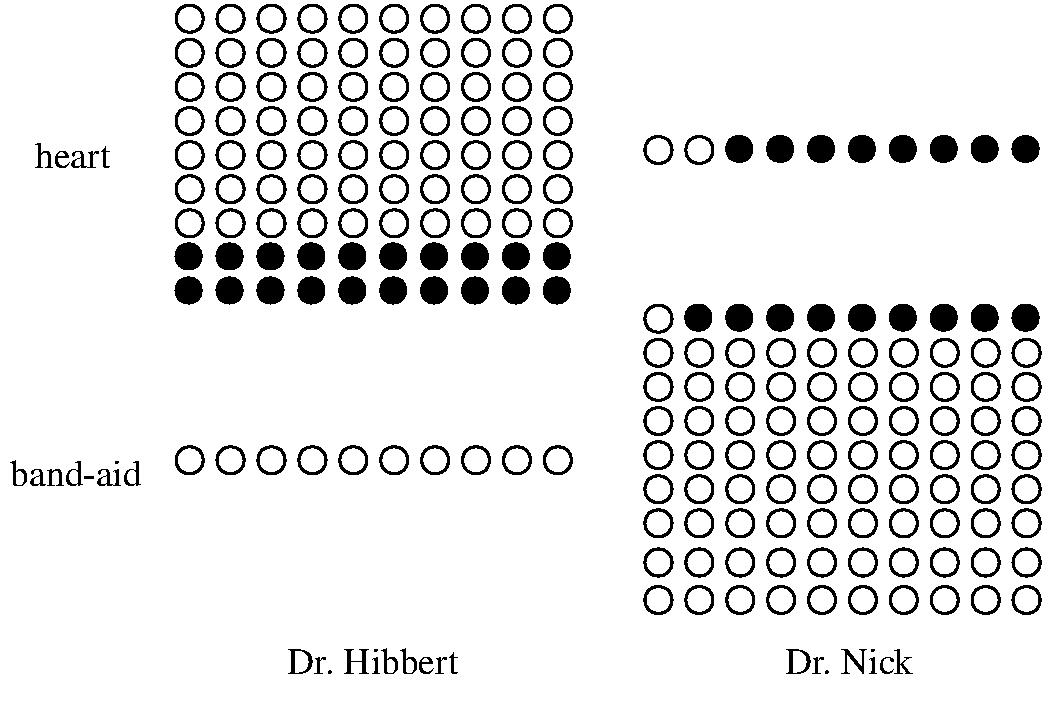
\includegraphics[width=2in]{figures/SimpsonsParadox.pdf}
%        \end{minipage}
% It is possible to have
%\[P(A\mid B,C) < P(A\mid B^c, C) \textnormal{ and } P(A\mid B, C^c) < P(A \mid B^c, C^c)\]
%\[ \textnormal{yet also } P(A\mid B) > P(A \mid B^c).\]
    
\subsection{Law of Total Probability (LOTP)}
Let ${ B}_1, { B}_2, { B}_3, ... { B}_n$ be a \emph{partition} of the sample space (i.e., they are disjoint and their union is the entire sample space).
   \[ P({ A}) = P({ A} \cap { B}_1)+ P({ A} \cap { B}_2)+ \dots + P({ A} \cap { B}_n) \]

Special case of LOTP with ${ B}$ and ${ B^c}$ as partition: 
 \[ P({ A}) = P({ A} \cap { B})+ P({ A} \cap { B^c}) \]
   
\subsection{Bayes' Rule}
If $ A_1,A_2, \dots , A_n $ form a partition of the Sample Space, S, and B is any event, then:
         \[P({ A_j}|{ B}) = \frac{P(A_j \cap B)}{P(B)} = \frac{P({ A_j})P({ B}|{ A_j})}{P({ B})} = \frac{P({ A_j})P({ B}|{ A_j})}{ \sum_{i=1}^{n} P({ A_i}) P(B | A_i) }  \]
         \[P({ A}|{ B} \cap { C}) = \frac{P({ B}|{ A} \cap { C})P({ A} | { C})}{P({ B} | { C})}\]
         We can also write
         $$P(A|B\cap C) = \frac{P(A \cap B \cap C)}{P(B \cap C)} = \frac{P(B\cap C|A)P(A)}{P(B\cap C)}$$
%\textbf{Odds Form of Bayes' Rule}
%\[\frac{P({ A}| { B})}{P({ A^c}| { B})} = \frac{P({ B}|{ A})}{P({ B}| { A^c})}\frac{P({ A})}{P({ A^c})}\]
%The \emph{posterior odds} of $A$ are the \emph{likelihood ratio} times the \emph{prior odds}. 

\section{Random Variables and their Distributions} \hrule height 2pt

% \subsection{Conditioning is the Soul of Statistics}

% Law of Total Probability with ${\bf B}$ and ${\bf B^c}$ (special case of a partitioning set), and with Extra Conditioning (just add C!)
%    \begin{align*} 
% P({\bf A}) &= P({\bf A} | {\bf B})P({\bf B}) + P({\bf A} | {\bf B^c})P({\bf B^c}) \\
% P({\bf A}) &= P({\bf A} \cap {\bf B})+ P({\bf A} \cap {\bf B^c}) \\
% P({\bf A} | {\bf C}) &= P({\bf A} | {\bf B}, {\bf C})P({\bf B} | {\bf C}) + P({\bf A} | {\bf B^c}, {\bf C})P({\bf B^c} | {\bf C}) \\
% P({\bf A} | {\bf C}) &= P({\bf A} \cap {\bf B} | {\bf C})+ P({\bf A} \cap {\bf B^c} | {\bf C})
%    \end{align*} 
   
% Law of Total Probability with a partitioning ${\bf B}_0, {\bf B}_1, {\bf B}_2, {\bf B}_3, \dots, {\bf B}_n$, and applied to random variables ${\bf X}$, ${\bf Y}$.
% \begin{align*} 
% P({\bf A}) &= \sum_{i=0}^n P({\bf A} | {\bf B}_i)P({\bf B}_i) \\
% P({\bf Y}=y) &= \sum_{k}P({\bf Y}=y|{\bf X}=k)P({\bf X}=k)
%    \end{align*} 
% Bayes' Rule, and with Extra Conditioning (just add C!)
%     \begin{align*}
%          P({\bf A}|{\bf B}) &= \frac{P({\bf A} \cap {\bf B})}{P({\bf B})} = \frac{P({\bf B}|{\bf A})P({\bf A})}{P({\bf B})} \\
%          P({\bf A}|{\bf B}, {\bf C}) &= \frac{P({\bf A} \cap {\bf B} | {\bf C})}{P({\bf B} | {\bf C})} = \frac{P({\bf B}|{\bf A}, {\bf C})P({\bf A} | {\bf C})}{P({\bf B} | {\bf C})} 
%     \end{align*}
    
\subsection{PMF, CDF, and Independence}
\begin{description}

\item[The Probability Mass Function (pmf)]
Gives the probability that a \emph{discrete} random variable takes on the value $x$.
\[ f(x) \equiv P(X=x) \]


\begin{minipage}{.45\linewidth}
            \centering
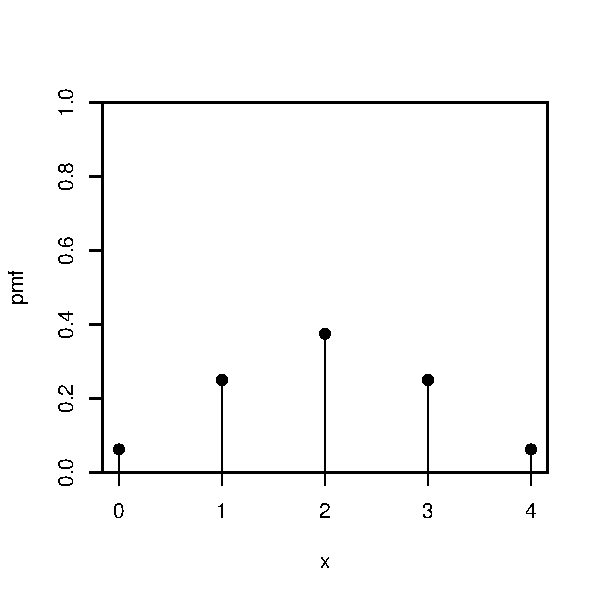
\includegraphics[width=1\linewidth, height=0.2\textheight]{figures/Binpmf.pdf}
        \end{minipage} %
   	 \begin{minipage}{.45\linewidth}
    	\centering
    	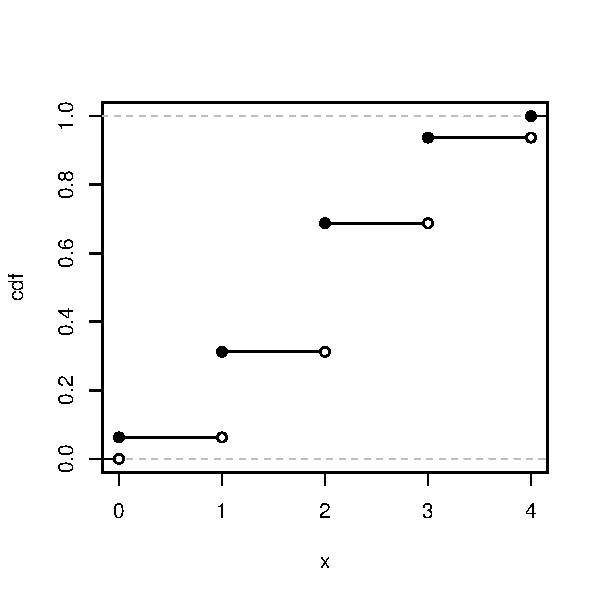
\includegraphics[width=1\linewidth, height=0.2\textheight]{figures/Bincdf.pdf}
    \end{minipage}


The PMF satisfies $f(x) \geq 0 \textrm{ and } \sum_x f(x) = 1 $.


The \textbf{Cumulative Distribution Function (cdf)} gives the probability that a random variable is less than or equal to $x$.
\[F_X(x) = P(X \leq x)\]


The CDF is an increasing, right-continuous function with
\[F_X(x) \to 0 \textrm{ as $x \to -\infty$ and } F_X(x) \to 1 \textrm{ as $x \to \infty$} \]
\item[Independence] Intuitively, two random variables are independent if knowing the value of one gives  no information about the other. Discrete r.v.s $X$ and $Y$ are independent if for \emph{all} values of $x$ and $y$  \begin{center}
$P(X=x \cap Y=y) = P(X = x)P(Y = y)$
\end{center}

\end{description}

\section{Expected Value} \hrule height 2pt 

\begin{description}
\item[Expected Value] (a.k.a.~\emph{mean}, \emph{expectation}, or \emph{average}) is a weighted average of the possible outcomes of our random variable. Mathematically, if $x_1, x_2, x_3, \dots$ are all of the distinct possible values that $X$ can take, the expected value of $X$ is
\begin{center}
$E(X) = \sum_{i} x_i P(X=x_i) = \mu$
\end{center}

%\begin{minipage}{\linewidth}
%            \centering
%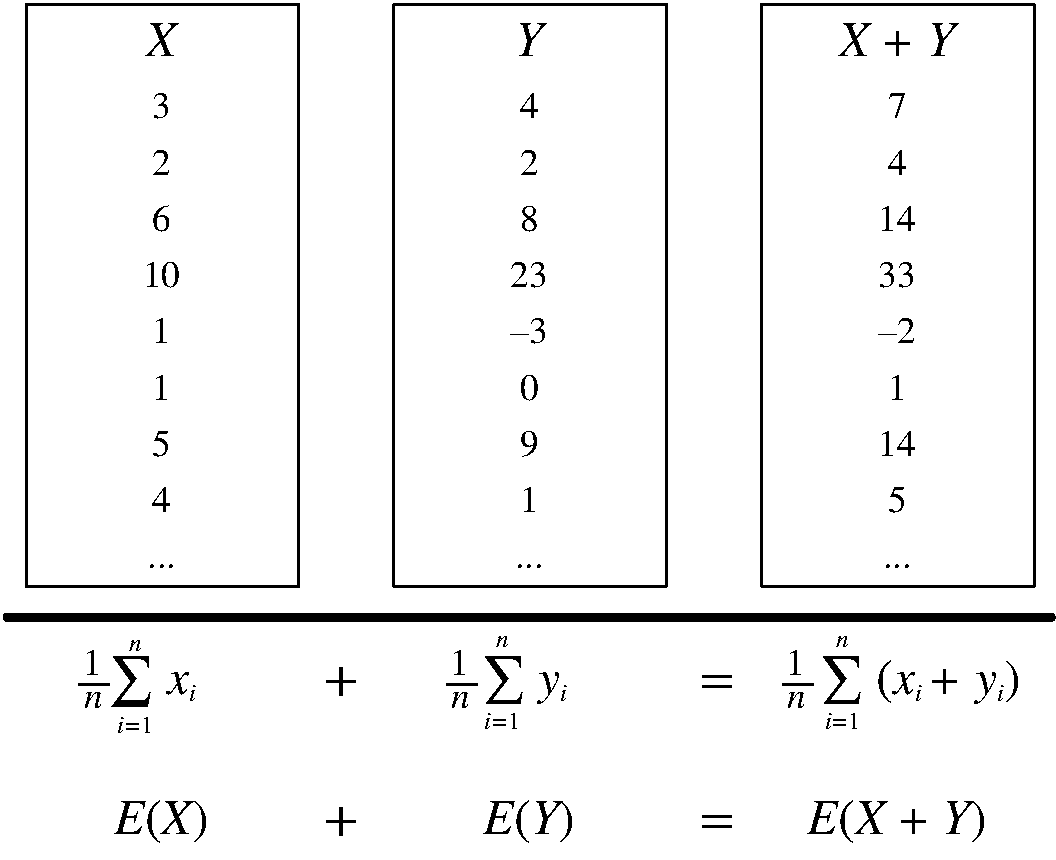
\includegraphics[width=2in]{figures/linearity.pdf}
%        \end{minipage}


\item[Linearity] For any r.v.s $X$ and $Y$, and constants $a,b,c,$ 
\[E(aX + bY + c) = aE(X) + bE(Y) + c \]

\item[Same distribution implies same mean] If $X$ and $Y$ have the same distribution, then $E(X)=E(Y)$ and, more generally, $E(g(X)) = E(g(Y))$


\item[Conditional Expected Value] is defined like expectation, only conditioned on any event $A$. \begin{center}
$\ E(X | A) = \sum_x x P(X=x | A)$
\end{center}

\end{description}

%\subsection{Indicator Random Variables}
%\begin{description}
%\item[Indicator Random Variable] is a random variable that takes on the value 1 or 0. It is always an indicator of some event: if the event occurs, the indicator is 1; otherwise it is 0. They are useful for many problems about counting how many events of some kind occur. Write \[
%I_A =
% \begin{cases}
%   1 & \text{if $A$ occurs,} \\
%   0 & \text{if $A$ does not occur.}
%  \end{cases}
%\]
%Note that $I_A^2 = I_A, I_A I_B = I_{A \cap B}, $ and $I_{A \cup B} = I_A + I_B - I_A I_B$. 
%\item[Distribution] $I_A \sim \Bern(p)$ where $p = P(A)$.
%\item[Fundamental Bridge] The expectation of the indicator for event $A$ is the probability of event $A$: $E(I_A) = P(A)$. 
%\end{description}

\subsection{Variance and Standard Deviation}

\[\var(X) = E \left(X - E(X)\right)^2 = E(X^2) - (E(X))^2 =\sigma^2 \]
\[\textrm{SD}(X) = \sqrt{\var(X)} = \sigma \]


\section{Continuous RVs, LOTUS,  UoU} \hrule height 2pt

\subsection{Continuous Random Variables (CRVs)}
\begin{description}
% \item[What is a Continuous Random Variable (CRV)?] A continuous random variable can take on any possible value within a certain interval (for example, [0, 1]), whereas a discrete random variable can only take on variables in a list of countable values (for example, all the integers, or the values 1, $\frac{1}{2}, \frac{1}{4}, \frac{1}{8}$, etc.)
% \item[Do Continuous Random Variables have PMFs?] No. The probability that a continuous random variable takes on any specific value is 0.
%\item[What's the probability that a CRV is in an interval?] Take the difference in CDF values (or use the PDF as described later).
%\[P(a \leq X \leq b) = P(X \leq b) - P(X \leq a) = F_X(b) - F_X(a)\]
%
%For $X \sim \N(\mu,\sigma^2)$, this becomes
%\begin{align*}
%P(a\leq X\leq b)&=\Phi \left(\frac{b-\mu }{\sigma } \right) - \Phi \left( \frac{a-\mu }{\sigma } \right)
%\end{align*}

\item[What is the Probability Density Function (PDF)?] The PDF $f$ is the derivative of the CDF $F$.
\[ F'(x) = f(x) \]
A PDF is nonnegative and integrates to $1$. By the fundamental theorem of calculus, to get from PDF back to CDF we can integrate:
\begin{align*} 
    F(x) &=  \int_{-\infty}^x f(t)dt  
   \end{align*}
   \begin{minipage}{\linewidth}
            \centering
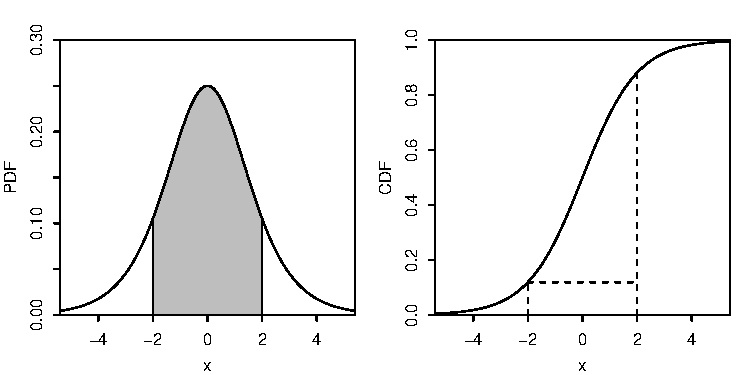
\includegraphics[width=2in]{figures/Logisticpdfcdf.pdf}
        \end{minipage}
   To find the probability that a CRV takes on a value in an interval, integrate the PDF over that interval.
      \begin{align*} 
    F(b) - F(a)  &=  \int^b_a f(x)dx
       \end{align*}
   


% Two additional properties of a PDF:  it must integrate to 1 (because the probability that a CRV falls in the interval $[-\infty, \infty]$ is 1, and the PDF must always be nonnegative.
% \[\int^\infty_{-\infty}f(x)dx \hspace{2 cm} f(x) \geq 0\]
\item[How do I find the expected value of a CRV?] Analogous to the discrete case, where you sum $x$ times the PMF, for CRVs you integrate $x$ times the PDF.
\[E(X) = \int^\infty_{-\infty}xf(x)dx \]
% Review: Expected value is \emph{linear}. This means that for \emph{any} random variables $X$ and $Y$ and any constants $a, b, c$, the following is true:
% \[E(aX + bY + c) = aE(X) + bE(Y) + c\]
\end{description}


\label{lotus}
\subsection{LOTUS}
\begin{description}
\item[Expected value of a function of an r.v.]
The expected value of $X$ is defined this way:
\[E(X) = \sum_x xP(X=x) \textnormal{ (for discrete $X$)}\]
\[E(X) = \int^\infty_{-\infty}xf(x)dx  \textnormal{ (for continuous $X$)}\]
The \textbf{Law of the Unconscious Statistician (LOTUS)} states that you can find the expected value of a \emph{function of a random variable}, $h(X)$, in a similar way, by replacing the $x$ in front of the PMF/PDF by $h(x)$ but still working with the PMF/PDF of $X$:
\[E(h(X)) = \sum_x h(x)P(X=x) \textnormal{ (for discrete $X$)}\]
\[E(h(X)) = \int^\infty_{-\infty}h(x)f(x)dx \textnormal{ (for continuous $X$)}\]
%\item[What's a function of a random variable?] A function of a random variable is also a random variable. For example, if $X$ is the number of bikes you see in an hour, then $g(X) =  2X$ is the number of bike wheels you see in that hour and $h(X) = {X \choose 2} = \frac{X(X-1)}{2}$ is the number of \emph{pairs} of bikes such that you see both of those bikes in that hour.
%\item[What's the point?] You don't need to know the PMF/PDF of $g(X)$ to find its expected value. All you need is the PMF/PDF of $X$. 
\end{description}

%\subsection{Universality of Uniform (UoU)} When you plug any CRV into its own CDF, you get a Uniform(0,1) random variable. When you plug a Uniform(0,1) r.v.~into an inverse CDF, you get an r.v.~with that CDF. For example, let's say that a random variable $X$ has CDF
%    \[ F(x) = 1 - e^{-x}, \textrm{ for $x>0$} \]
%    By  UoU, if we plug $X$ into this function then we get a uniformly distributed random variable.
%    \[ F(X) = 1 - e^{-X} \sim \textrm{Unif}(0,1)\]
%    Similarly, if $U \sim \textrm{Unif}(0,1)$ then $F^{-1}(U)$ has CDF $F$. The key point is that {for any continuous random variable $X$, we can transform it into a Uniform random variable and back by using its CDF.}

\section{Moments and MGFs} \hrule height 2pt

\subsection{Moments}
Let $X$ have mean $\mu$ and standard deviation $\sigma$, then: \\

The $ k^{th}$ \textbf{moment} of a RV, $ X $, is $ E[X^k] = \SumInt x^k f(x) $.\\
The $ k^{th}$ \textbf{central moment} of a RV, $ X $, is $ E[(X-\mu)^k] = \SumInt (x-\mu)^k f(x) $.

The mean and variance are important summaries of the shape of a distribution.
    \begin{description}
        \item[Mean] $E(X) = \mu_1 $
        \item[Variance] $\var(X) = \mu_2 - \mu_1^2$
%        \item[Skewness] $\textrm{Skew}(X) = m_3$
%      \item[Kurtosis] $\textrm{Kurt}(X) = m_4 - 3$
    \end{description}

\subsection{Moment Generating Functions}

\begin{description}
    \item[MGF] For any random variable $X$, the function
        \[ M_X(t) = E(e^{tX}) \]
        is the \textbf{moment generating function (MGF)} of $X$, if it exists for all $t$ in some open interval containing $0$.
                
%            \item[Why is it called the Moment Generating Function?] Because the $k$th derivative of the moment generating function, evaluated at $0$, is the $k$th moment of $X$.
%    \[\mu_k = E(X^k) = M_X^{(k)}(0)\]
%    This is true by Taylor expansion of $e^{tX}$ since
%    \[M_X(t) = E(e^{tX}) = \sum_{k=0}^\infty \frac{E(X^k)t^k}{k!} = \sum_{k=0}^\infty \frac{\mu_k t^k}{k!} \]
%
    \item[MGF of linear functions] If we have $Y = aX + b$, then
        \[M_Y(t) = E(e^{t(aX + b)}) =  e^{bt}E(e^{(at)X}) = e^{bt}M_X(at)\]
       
%    \item[Uniqueness] \emph{If it exists, the MGF uniquely determines the distribution}. This means that for any two random variables $X$ and $Y$, they are distributed the same (their PMFs/PDFs are equal) if and only if their MGFs are equal. 
    \item[Summing Independent RVs by Multiplying MGFs.] If $X$ and $Y$ are independent, then
    \begin{align*}
        M_{X+Y}(t) &= E(e^{t(X + Y)}) = E(e^{tX})E(e^{tY}) = M_X(t) \cdot M_Y(t) 
    \end{align*}
    The MGF of the sum of two random variables is the product of the MGFs of those two random variables.
\end{description}

\section{Joint PDFs and CDFs} \hrule height 2pt 

\subsection{Joint Distributions}
The \textbf{joint CDF} of $X$ and $Y$ is 
$$F(x,y)=P(X \leq x, Y \leq y)$$
In the discrete case, $X$ and $Y$ have a \textbf{joint PMF} 
$$p_{X,Y}(x,y) = P(X=x,Y=y).$$ In the continuous case, they have a \textbf{joint PDF}
\[f_{X,Y}(x,y) = \frac{\partial^2}{\partial x \partial y} F_{X,Y}(x,y).\]
The joint PMF/PDF must be nonnegative and sum/integrate to 1.
%\begin{minipage}{\linewidth}
%            \centering
%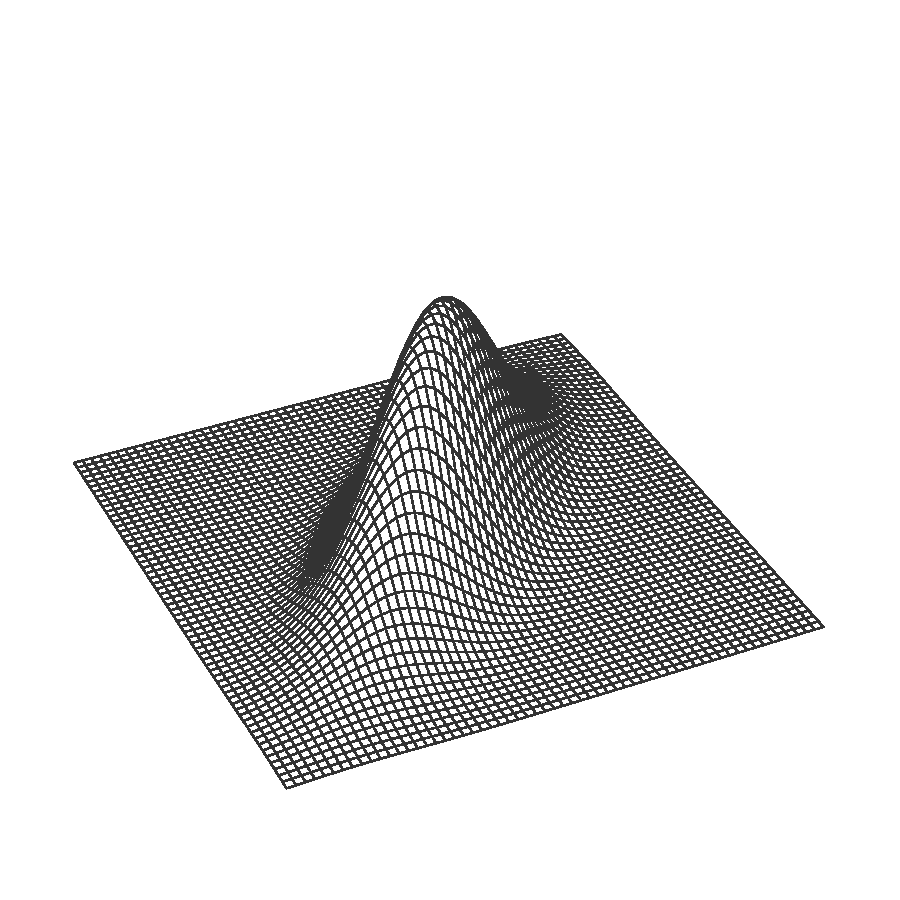
\includegraphics[width=1.0in]{figures/jointPDF.pdf}
%        \end{minipage}
\subsection{Conditional Distributions}
\textbf{Conditioning and Bayes' rule for discrete r.v.s}
\[P(Y=y|X=x) = \frac{P(X=x, Y=y)}{P(X=x)} = \frac{P(X=x|Y=y)P(Y=y)}{P(X=x)}\]
\textbf{Conditioning and Bayes' rule for continuous r.v.s}
\[f_{Y|X}(y|x) = \frac{f_{X,Y}(x, y)}{f_X(x)} = \frac{f_{X|Y}(x|y)f_Y(y)}{f_X(x)}\]
%\textbf{Hybrid Bayes' rule}
%\[f_X(x|A) = \frac{P(A | X = x)f_X(x)}{P(A)}\]

\subsection{Marginal Distributions}
To find the distribution of one (or more) random variables from a joint PMF/PDF, sum/integrate over the unwanted random variables. \medskip

\textbf{Marginal PMF from joint PMF}
\[P(X = x) = \sum_y P(X=x, Y=y)\]
\textbf{Marginal PDF from joint PDF}
\[f_X(x) = \int_{-\infty}^\infty f_{X, Y}(x, y) dy\]

\textbf{Limits of marginals and expected values:} Note that the only time you are integrating over \textit{all} the possible values of $ Y $ for the continuous case is when you are trying to find its expected value. \\
For example, given iid RV's $ X,Y$, w/ pdf $ f(x,y)=3x,\ 0<y<x<1 $

$ \Rightarrow E[X] = \int_{- \infty}^{\infty} xf_X (x) dx = \int_{- \infty}^{\infty} x[ \int_{- \infty}^{\infty } f(x,y) dy ] dx =  \int_{- \infty}^{\infty}x [ \int_{0}^{x} 3x dy ] dx =  \int_{- \infty}^{\infty} x [ 3x^2,\ 0<x<1 ] dx = \int_{0}^{1} x3x^2 dx = \frac{3}{4} $  

However note that $ E[XY] = \int_{-\infty}^{\infty} \int_{-\infty}^{\infty} xy\ f(x,y)\ dy\ dx $, which using the previous joint pdf: $ = \int_{0}^{1} \int_{0}^{x} xy\ 3x\ dy\ dx $


\subsection{Independence of Random Variables}
Random variables $X$ and $Y$ are independent if and only if any of the following conditions holds:
\begin{itemize}
    \itemsep -1mm
    \item Joint CDF is the product of the marginal CDFs 
    \item Joint PMF/PDF is the product of the marginal PMFs/PDFs
    \item Conditional distribution of $Y$ given $X$ is the marginal distribution of $Y$
    \item ie no funny limits, and pdf/cdf/pmf's \textit{can} be factored out
\end{itemize}
% Write $X \independent Y$ to denote that $X$ and $Y$ are independent.

\subsection{Multivariate LOTUS}
LOTUS in more than one dimension is analogous to the 1D LOTUS.
For discrete random variables:
\[E(g(X, Y)) = \sum_x\sum_yg(x, y)P(X=x, Y=y)\]
For continuous random variables:
\[E(g(X, Y)) = \int_{-\infty}^{\infty}\int_{-\infty}^{\infty}g(x, y)f_{X,Y}(x, y)dxdy\]

\section{Covariance and Transformations} \hrule height 2pt 

\subsection{Covariance and Correlation}
\begin{description}
\item [Covariance] is the analog of variance for two random variables.
    \[\cov(X, Y) = E\left((X - E(X))(Y - E(Y))\right) = E(XY) - E(X)E(Y)\]
    Note that 
    \[\cov(X, X) = E(X^2) - (E(X))^2 =  \var(X)\]
\item [Correlation] is a standardized version of covariance that is always between $-1$ and $1$.
    \[\corr(X, Y) = \frac{\cov(X, Y)}{\sqrt{\var(X)\var(Y)}} \]
\item [Covariance and Independence] If two random variables are independent, then they are uncorrelated. The converse is not necessarily true (e.g., consider $X \sim \N(0,1)$ and $Y=X^2$).
    \begin{align*}
    	X \independent Y &\longrightarrow \cov(X, Y) = 0 \longrightarrow E(XY) = E(X)E(Y)
    \end{align*}
%, except in the case of Multivariate Normal, where uncorrelated \emph{does} imply independence.
\item [Covariance and Variance]  The variance of a sum can be found by
    \begin{align*}
        %\cov(X, X) &= \var(X) \\
        \var(X + Y) &= \var(X) + \var(Y) + 2\cov(X, Y) \\
        \var(X_1 + X_2 + \dots + X_n ) &= \sum_{i = 1}^{n}\var(X_i) + 2\sum_{i < j} \cov(X_i, X_j)
    \end{align*}
    If $X$ and $Y$ are independent then they have covariance $0$, so
    \[X \independent Y \Longrightarrow \var(X + Y) = \var(X) + \var(Y)\]
%    If $X_1, X_2, \dots, X_n$ are identically distributed and have the same covariance relationships (often by \textbf{symmetry}), then 
%    \[\var(X_1 + X_2 + \dots + X_n ) = n\var(X_1) + 2{n \choose 2}\cov(X_1, X_2)\]
\item [Covariance Properties]  For random variables $W, X, Y, Z$ and constants $a, b$:
    \begin{align*}
    	\cov(X, Y) &= \cov(Y, X) \\
        \cov(X + a, Y + b) &= \cov(X, Y) \\
        \cov(aX, bY) &= a*b*\cov(X, Y) \\
        \cov(W + X, Y + Z) &= \cov(W, Y) + \cov(W, Z)\\
        &\quad + \cov(X, Y) + \cov(X, Z)
    \end{align*}
\item [Correlation is location-invariant and scale-invariant] For any constants $a,b,c,d$ with $a$ and $c$ nonzero,
   \[ \corr(aX + b, cY + d) = \corr(X, Y) \]
\end{description}%

\subsection{Transformations}
\begin{description}
    \label{one variable transformations}
    \item[One Variable Transformations] Let's say that we have a random variable $X$ with PDF $f_X(x)$, but we are also interested in some function of $X$. We call this function $Y = g(X)$. Also let $y=g(x)$. If $g$ is differentiable and strictly increasing (or strictly decreasing), then the PDF of $Y$ is
    \[f_Y(y) = f_X(x)\left|\frac{dx}{dy}\right| =  f_X(g^{-1}(y))\left|\frac{d}{dy}g^{-1}(y)\right|\]
    The derivative of the inverse transformation is called the \textbf{Jacobian}.
\end{description}%

%\section{Table of Distributions} \hrule height 2pt
%
%\begin{center}
%	\tiny
%	%\renewcommand{\arraystretch}{3.6}
%	\begin{tabular}{ccccZ}
%		\textbf{Distribution} & \textbf{PMF/PDF and Support} & $ \mathbf{ E[X] } $  & $ \textbf{Var(X)} $ & \textbf{MGF}\\
%		\hline 
%		\shortstack{Bernoulli \\ \Bern($p$)} & \shortstack{$P(X=1) = p$ \\$ P(X=0) = q=1-p$} & $p$ & $pq$ & $q + pe^t$ \\
%		\hline
%		\shortstack{Binomial \\ \Bin($n, p$)} & \shortstack{$P(X=k) = {n \choose k}p^k q^{n-k}$  \\ $k \in \{0, 1, 2, \dots n\}$}& $np$ & $npq$ & $(q + pe^t)^n$ \\
%		\hline
%		\shortstack{Geometric \\ \Geom($p$)} & \shortstack{$P(X=k) = q^kp$  \\ $k \in \{$0, 1, 2, \dots $\}$}& $q/p$ & $q/p^2$ & $\frac{p}{1-qe^t}, \, qe^t < 1$\\
%		\hline
%		\shortstack{Negative Binomial \\ \NBin($r, p$)} & \shortstack{$P(X=n) = {r + n - 1 \choose r -1}p^rq^n$ \\ $n \in \{$0, 1, 2, \dots $\}$} & $rq/p$ & $rq/p^2$ &  $(\frac{p}{1-qe^t})^r, \, qe^t < 1$\\
%		\hline
%		\shortstack{Hypergeometric \\ \Hypergeometric($w, b, n$)} & \shortstack{$P(X=k) = \sfrac{{w \choose k}{b \choose n-k}}{{w + b \choose n}}$ \\ $k \in \{0, 1, 2, \dots,  n\}$} & $\frac{nw}{b+w}$ & messy & messy  \\
%		\hline
%		\shortstack{Poisson \\ \Pois($\lambda$)} & \shortstack{$P(X=k) = \frac{e^{-\lambda}\lambda^k}{k!}$ \\ $k \in \{$0, 1, 2, \dots $\}$} & $\lambda$ & $\lambda$ & $e^{\lambda(e^t-1)}$ \\
%		\hline
%		\hline
%		\shortstack{Uniform \\ \Unif($a, b$)} & \shortstack{$ f(x) = \frac{1}{b-a}$ \\$ x \in (a, b) $} & $\frac{a+b}{2}$ & $\frac{(b-a)^2}{12}$ &  $\frac{e^{tb}-e^{ta}}{t(b-a)}$\\
%		\hline
%		\shortstack{Normal \\ $\N(\mu, \sigma^2)$} & \shortstack{$f(x) = \frac{1}{\sigma \sqrt{2\pi}} e^{-\sfrac{(x - \mu)^2}{(2 \sigma^2)}}$ \\ $x \in (-\infty, \infty)$} & $\mu$  & $\sigma^2$ & $e^{t\mu + \frac{\sigma^2t^2}{2}}$\\
%		\hline
%		\shortstack{Exponential \\ $\Expo(\lambda)$} & \shortstack{$f(x) = \lambda e^{-\lambda x}$\\$ x \in (0, \infty)$} & $\frac{1}{\lambda}$  & $\frac{1}{\lambda^2}$ & $\frac{\lambda}{\lambda - t}, \, t < \lambda$\\
%		\hline
%	\end{tabular}
%\end{center}

\section{Useful Facts}  \hrule height 2pt

\subsection{Convolutions of Random Variables}
A convolution of $n$ random variables is simply their sum. For the following results, let $X$ and $Y$ be \emph{independent}.
\begin{enumerate}
	\itemsep -.5mm
	\item  $X \sim \Pois(\lambda_1)$, $Y \sim \Pois(\lambda_2)$ $\longrightarrow X + Y \sim \Pois(\lambda_1 + \lambda_2)$
	\item  $X \sim \Bin(n_1, p)$, $Y \sim \Bin(n_2, p)$ $\longrightarrow X + Y \sim \Bin(n_1 + n_2, p)$. $\Bin(n,p)$ can be thought of as a sum of i.i.d.~$\Bern(p)$ r.v.s.
	\item  $X \sim \Gam(a_1, \lambda)$, $Y \sim \Gam(a_2, \lambda)$ $\longrightarrow  X + Y \sim\Gam(a_1 + a_2, \lambda)$.  $\Gam(n,\lambda)$ with $n$ an integer can  be thought of as a sum of i.i.d.~Expo($\lambda$) r.v.s.
	\item  $X \sim \NBin(r_1, p)$, $Y \sim \NBin(r_2, p)$ $\longrightarrow  X + Y \sim\NBin(r_1 + r_2, p)$. $\NBin(r,p)$ can  be thought of as a sum of i.i.d.~Geom($p$) r.v.s.
	\item  $X \sim \N(\mu_1, \sigma_1^2)$, $Y \sim \N(\mu_2, \sigma_2^2)$  $\longrightarrow  X + Y \sim \N(\mu_1 + \mu_2, \sigma_1^2 + \sigma_2^2)$
\end{enumerate}
\vspace*{-.15cm}
\subsection{Special Cases of Distributions}
\begin{enumerate}
	\itemsep -.5mm
	\item $\Bin(1, p) \sim \Bern(p)$
	\item $\Beta(1, 1) \sim \Unif(0, 1)$
	\item $\Gam(1, \lambda) \sim \Expo(\lambda)$
	\item $\chi^2_n \sim \Gam\left(\frac{n}{2}, \frac{1}{2}\right)$
	\item $\NBin(1, p) \sim \Geom(p)$
\end{enumerate}

\vspace*{-.25cm}
\subsection{Inequalities}

\begin{enumerate}
	\itemsep -.5mm
	\item \textbf{Cauchy-Schwarz} $|E(XY)| \leq \sqrt{E(X^2)E(Y^2)}$
	\item \textbf{Markov} $P(X \geq a) \leq \frac{E|X|}{a}$ for $a>0$
	\item \textbf{Chebyshev} $P(|X - \mu| \geq a) \leq \frac{\sigma^2}{a^2}$ for $E(X)=\mu, \var(X) = \sigma^2$
	\item \textbf{Jensen} $E(g(X)) \geq g(E(X))$ for $g$ convex; reverse if $g$ is concave
	\item \textbf{Chebychev's Inequality}: gives rough bounds on certain probabilities.\\
	$ E[X]=\mu, V(X)=\sigma^2 \Rightarrow \forall \varepsilon >0,\ P(|X-\mu| \geq \varepsilon) \leq \frac{\sigma^2}{\varepsilon^2}  $	
\end{enumerate}


%	\item[Failure rate function] Definition: If X is a cts RV with pdf f(x) and cdf F(x), then its failure rate function is 
%	
%		\[ S(t) \equiv \frac{f(t)}{P(X>t)} = \frac{f(t)}{1-F(t)} \]
%	which can loosely be regarded as X’s instantaneous rate of death, given that it has so far survived to time t.

%\item[Definition] We have a \textbf{Poisson process} of rate $\lambda$ arrivals per unit time if the following conditions hold:
%	\begin{enumerate}
%		\item The number of arrivals in a time interval of length $t$ is $\Pois(\lambda t)$.
%		\item Numbers of arrivals in disjoint time intervals are independent.
%	\end{enumerate}



\section{Conditional Expectation} \hrule height 2pt
\begin{description}
	%\itemsep -.5mm
	\item[Conditioning on an Event] We can find $E(Y|A)$, the expected value of $Y$ given that event $A$ occurred. A very important case is when $A$ is the event $X=x$. Note that $E(Y|A)$ is a \emph{number}. For example: 
	\begin{itemize}
		\itemsep -.5mm
		\item The expected value of a fair die roll, given that it is prime, is $\frac{1}{3} \cdot 2 + \frac{1}{3} \cdot 3 + \frac{1}{3} \cdot 5 = \frac{10}{3}$.
		\item Let $Y$ be the number of successes in $10$ independent Bernoulli trials with probability $p$ of success. Let $A$ be the event that the first $3$ trials are all successes. Then
		$$E(Y|A) = 3 + 7p$$
		since the number of successes among the last $7$ trials is $\Bin(7,p)$. 
		\item Let $T \sim \Expo(1/10)$ be how long you have to wait until the shuttle comes. Given that you have already waited $t$ minutes, the expected additional waiting time is 10 more minutes, by the memoryless property. That is, $E(T|T>t) = t + 10$.
	\end{itemize}
\end{description}
\begin{center}
\scalebox{0.85}{
	\setlength{\extrarowheight}{7pt}
	\begin{tabular}{ccc}
		\textbf{Discrete $Y$} & \textbf{Continuous $Y$} \\
		\toprule
		$E(Y) = \sum_y yP(Y=y)$ & $E(Y) =\int_{-\infty}^\infty yf_Y(y)dy$ \\
		% $E(Y|X=x) = \sum_y yP(Y=y|X=x)$ & $E(Y|X=x) =\int_{-\infty}^\infty yf_{Y|X}(y|x)dy$ \\
		$E(Y|A) = \sum_y yP(Y=y|A)$ & $E(Y|A) = \int_{-\infty}^\infty yf(y|A)dy$ \\ 
		\bottomrule
	\end{tabular}
}
\end{center}
\begin{description}
	\item[Conditioning on a Random Variable]  We can also find $E(Y|X)$, the expected value of $Y$ given the random variable $X$. This is \emph{a function of the random variable $X$}. It is \emph{not} a number except in certain special cases such as if $X \independent Y$. To find $E(Y|X)$, find $E(Y|X = x)$ and then plug in $X$ for $x$. For example:
	\begin{itemize}
		\itemsep -.5mm
		\item If $E(Y|X=x) = x^3+5x$, then $E(Y|X) = X^3 + 5X$.
		\item Let $Y$ be the number of successes in $10$ independent Bernoulli trials with probability $p$ of success and $X$ be the number of successes among the first $3$ trials. Then $E(Y|X)=X+7p$.
		\item Let $X \sim \N(0,1)$ and $Y=X^2$. Then $E(Y|X=x) = x^2$ since if we know $X=x$ then we know $Y=x^2$. And $E(X|Y=y) = 0$ since if we know $Y=y$ then we know $X = \pm \sqrt{y}$, with equal probabilities (by symmetry). So $E(Y|X)=X^2, E(X|Y)=0$.  
	\end{itemize} 
	
	\item[Properties of Conditional Expectation] \quad
	\begin{enumerate}
		\item $E(Y|X) = E(Y)$ if $X \independent Y$
		\item $E(h(X)W|X) = h(X)E(W|X)$ (\textbf{taking out what's known}) \\
		In particular, $E(h(X)|X) = h(X)$.
		\item $E(E(Y|X)) = E(Y)$ (\textbf{Law of Iterated Expectation (LIE)}, a.k.a.~Law of Total Expectation, a.k.a.~Adam's Law)
	\end{enumerate}
	
	\item[Law of Iterated Expectation (LIE)]  can also be written in a way that looks analogous to \textbf{LOTP}. For any events $A_1, A_2, \dots, A_n$ that partition the sample space, 
	\begin{align*}
	E(Y) &= E(Y|A_1)P(A_1) + \dots + E(Y|A_n)P(A_n)
	\end{align*}
	For the special case where the partition is $A, A^c$, this says
	\begin{align*}
	E(Y) &= E(Y|A)P(A) + E(Y|A^c)P(A^c)
	\end{align*}
	
	\item[Eve's Law (a.k.a.~Law of Total Variance)] \quad
	\[\var(Y) = E(\var(Y|X)) + \var(E(Y|X))\]
\end{description}


%\subsection{Transformations}
%\begin{description}
%    \label{one variable transformations}
%    \item[One Variable Transformations] Let's say that we have a random variable $X$ with PDF $f_X(x)$, but we are also interested in some function of $X$. We call this function $Y = g(X)$. Also let $y=g(x)$. If $g$ is differentiable and strictly increasing (or strictly decreasing), then the PDF of $Y$ is
%    \[f_Y(y) = f_X(x)\left|\frac{dx}{dy}\right| =  f_X(g^{-1}(y))\left|\frac{d}{dy}g^{-1}(y)\right|\]
%    The derivative of the inverse transformation is called the \textbf{Jacobian}.
%
%
%     \item[Two Variable Transformations] Similarly, let's say we know the joint PDF of $U$ and $V$ but are also interested in the random vector $(X, Y)$ defined by $(X, Y) = g(U, V)$. Let 
%       $$  \frac{\partial (u,v)}{\partial (x,y)}  = \begin{pmatrix} 
%              \frac{\partial u}{\partial x} &  \frac{\partial u}{\partial y} \\
%           \frac{\partial v}{\partial x} & \frac{\partial v}{\partial y}   \\
%        \end{pmatrix}$$
%     be the \textbf{Jacobian matrix}. If the entries in this matrix exist and are continuous, and the determinant of the matrix is never $0$, then
%     \[f_{X,Y}(x, y) = f_{U,V}(u,v) \left|\left|   \frac{\partial (u,v)}{\partial (x,y)}\right| \right| \]
%   The inner bars tells us to take the matrix's determinant, and the outer bars tell us to take the absolute value.  In a $2 \times 2$ matrix, 
%     \[ \left| \left|
%     \begin{array}{ccc}
%         a & b \\
%         c & d
%     \end{array}
%     \right| \right| = |ad - bc|\]
%
%\end{description}
%
%\label{convolutions}
%\subsection{Convolutions}
%\begin{description}
%    \item[Convolution Integral] If you want to find the PDF of the sum of two independent CRVs $X$ and $Y$, you can do the following integral:
%        \[f_{X+Y}(t)=\int_{-\infty}^\infty f_X(x)f_Y(t-x)dx\]
%    \item[Example] Let $X,Y \sim \N(0,1)$ be i.i.d. Then for each fixed $t$,\[f_{X+Y}(t)=\int_{-\infty}^\infty \frac{1}{\sqrt{2\pi}}e^{-x^2/2} \frac{1}{\sqrt{2\pi}}e^{-(t-x)^2/2} dx\]
%By completing the square and using the fact that a Normal PDF integrates to $1$, this works out to $f_{X+Y}(t)$ being the $\N(0,2)$ PDF.
%\end{description}

\section{Method of Moments (MoM) Estimators}
\hrule height 2pt
MoM for
\begin{itemize}
	\itemsep -.5mm
	\item $ \mu = E[X_i] = \bar{X} = \frac{\sum_{i=1}^{n} X_i}{n} $
	\item $ E[X_i^2] \frac{\sum_{i=1}^{n} X_i}{n}  $
	\item $ Var(X_i)=E[X_i^2]-(E[X_i])^2 $
\end{itemize}

\subsection{$\chi^2$ (Chi-Square) Distribution}

Let us say that $X$ is distributed $\chi^2_n$. We know the following:
\begin{description}
	\item[Story] A Chi-Square($n$) is the sum of the squares of $n$ independent standard Normal r.v.s.
	%\item[Example]  The sum of squared errors are distributed $\chi^2_n$
	%     \item[PDF] The PDF of a $\chi^2_1$ is:
	% \begin{eqnarray*}
	% f(w) = \frac{1}{\sqrt{2\pi w}}e^{-w/2},
	% w \in [0, \infty)
	% \end{eqnarray*}
	\item[Properties and Representations]
	\[ Z_1 + Z_2 + \dots + Z_k \textrm{ for i.i.d.~$Z_i \sim \N(0,1)$} \Rightarrow Y=\sum_{i=1}^{k} Z_i^2 \sim \chi^2(k)   \]
\end{description}

\subsection{t-distribution}
suppose $ Z\sim N(0,1), Y\sim \chi^2 (k), Z \independent Y \Rightarrow T \equiv \frac{Z}{\sqrt{\frac{Y}{k}}} $

\subsection{F-Distribution}
	\begin{itemize}
		\itemsep -.5mm
		\item Suppose $ X \sim \chi^2(n),\ Y\sim \chi^2(m),\ X \independent Y \Rightarrow F \equiv \frac{\sfrac{X}{n}}{\sfrac{Y}{m}} \sim F(n,m) $. That is, the F-distribution is the ratio of two Chi-Squared Distributed variables divided by their respective degrees of freedom.
		\item $ E[F]=\frac{m}{m-2},\ m>2,\ Var(F) = \frac{\left(2 n+m-2\right) \sqrt{8\left(m-4\right)}}{\left(m-6\right) \sqrt{n\left(n+m-2\right)}} $
		\item $ F \sim F(n,m) \Rightarrow \text{we denote the } (1-\alpha)\text{ quantile by} F_{\alpha,n,m},\ ie\ P(F>F_{\alpha,n,m})=\alpha $
		\item $ F_{1-\alpha,m,n}=\frac{1}{F_{\alpha,n,m}} $
		\item Used for ratio of variances
	\end{itemize}


%\section{Confidence Intervals}
%\subsection{Known Variances}
%\[ 1-\alpha=P\Big(\bar{X} - z_{\frac{\alpha}{2}} \sqrt{\frac{\sigma^2}{n}} \leq \mu \leq \bar{X} + z_{\frac{\alpha}{2}} \sqrt{\frac{\sigma^2}{n}} \Big) \]\\
%\[ =P(L \leq \mu \leq U) \]
%We can write the interval as the \textit{Half-Width}: 
%\[ H \equiv z_{\frac{\alpha}{2}} \sqrt{\frac{\sigma^2}{n}}  \]
%If we want to solve for the \# of observations to for a wanted CI: 
%\[ z_{\frac{\alpha}{2}} \sqrt{\frac{\sigma^2}{n}} \leq \varepsilon \iff n\geq \Big( \frac{\sigma z_{\alpha/2}}{\varepsilon} \Big)^2  \]
%
%\textbf{1-sided 100(1-$ \alpha $)\% CI}
%\begin{align*}
%\text{Upper:} &\ \mu &\ \leq \bar{X} &\ + z_\alpha \sqrt{\sigma/n}\\
%\text{Lower:} &\ &\ \geq &\ -
%\end{align*}
%\subsection{Difference of means with known variances}
%\[ Z \equiv \frac{ \bar{X}-\bar{Y}-(\mu_x-\mu_y ) }{ \sqrt{ \sigma^2_x/n + \sigma^2_y/m } } \sim N(0,1)\ s.t.\ P(-z_\alpha/2 \leq z \leq z_\alpha/2  ) = 1-\alpha \]
%1-sided: 
%\begin{align*}
%\text{Upper:} &\ \mu_x-\mu_y &\ \leq \bar{X}-\bar{Y}  &\ + z_\alpha  \sqrt{ \sigma^2_x/n + \sigma^2_y/m }\\
%\text{Lower:} &\ &\ \geq &\ -
%\end{align*}
%Half Length: Assume n=m:
%\[ n \geq \frac{z^2_{\alpha/2}(\sigma^2_x+\sigma^2_y)}{\varepsilon^2} \]
%
%\subsection{Normal means with unknown variances}
%Facts:
%\begin{enumerate}
%	\itemsep -.5mm
%	\item $ \frac{\bar{X} - \mu}{\sqrt{\sigma^2/n}} \sim N(0,1) $
%	\item $ S^2 = \frac{\sum (X_i -\bar{X})^2}{n-1} \sim \frac{\sigma^2 \chi^2 (n-1)}{n-1} $
%	\item $ \bar{X} \independent S^2 $
%\end{enumerate}
%\[ \frac{\bar{X} - \mu}{\sqrt{S^2/n}} \sim t(n-1) \]
%2-sided: $ \mu \in \bar{X} \pm t_{\alpha/2,\ n-1} \sqrt{S^2/n} $\\
%1-sided:
%\begin{align*}
%\text{Upper:} &\ \mu &\ \leq \bar{X}  &\ + t_{\alpha,\ n-1}  \sqrt{ S^2/n }\\
%\text{Lower:} &\ &\ \geq &\ -
%\end{align*}
%Half-Length: $ H \equiv t_{\alpha/2,n-1}\sqrt{S^2/n} $
%
%\subsection{Difference of two normal means with unknown variance}
%Three Cases:\\
%\textbf{Case 1: $ \sigma^2_x = \sigma^2_y = \sigma^2 $:}
%In this case, we pool the variances:\\
%\[ S^2_p = \frac{(n-1)S^2_x + (m-1)S^2_y}{n+m-2} \sim \frac{\sigma^2 \chi^2 (n+m-2)}{n+m-2} \]
%\[ \frac{\bar{X} - \bar{Y} -(\mu_x -\mu_y)}{S_p^1 \sqrt{1/n + 1/m}} \sim t(n+m-2) \]
%2-sided: $ \mu_x-\mu_y \in \bar{X} \bar{Y} \pm t_{\alpha/2,n+m-2}S_p \sqrt{1/n+1/m} $\\
%1-sided: $ t_{\alpha,n+m-2} $; Upper: $ \leq,\ -  $, Lower: $ \geq,\ + $.\\
%\textbf{Case 2: Unequal variances:}
%\[ t^* \equiv \frac{\bar{X} - \bar{Y} - (\mu_x-\mu_y)}{\sqrt{S^2_x/n + S^2_y/m}} \sim \nu  \]
%\[ \nu \equiv \frac{(S^2_x/n + S^2_y/m)^2}{ \frac{(S^2_x/n)^2}{n+1} + \frac{(S^2_y/m)^2}{m+1} } -2 \]
%2-sided: $ \mu_x - \mu_y \in \bar{X} - \bar{Y} \pm t_{\alpha/2,\nu} \sqrt{S_x^2/n + S^2_y/m} $\\
%1-sided: $ t_{\alpha,\nu} $: Upper: $ \leq,\ + $ Lower: $ \geq,\ - $\\
%\textbf{NOTE:} We round down $ \nu $ to be conservative. \\
%\textbf{Case 3: Paired Normal Means:}\\
%Pair up $ X_i\ $ with $ Y_i $ s.t. $ X_i \independent Y_j $ but it need not be the case that $ X_i \not \independent Y_i $.\\
%Define the difference $ D_i \equiv X_i-Y_i $ s.t. $ D_1, D_2, \dots , D_n \overset{i.i.d.}{\sim} N(\mu,\ \sigma^2/n),\ \bar{D} \equiv \frac{\sum_{i = 1}^n D_i}{n},\ S^2_D \equiv \frac{\sum_{i = 1}^n (D_i \bar{D})^2}{n-1} \sim \frac{\sigma^2_D \chi^2(n-1)}{n-1} $
%\[ \frac{\bar{D} -\mu_d}{\sqrt{S_d^2/n}} \sim t(n-1) \]
%2-sided: $ \mu_d \in \bar{D} \pm t_{\alpha/2,n-1}\sqrt{S^2_d/n} $\\
%1-sided $ t_{\alpha,n-1} $ Upper: $ \leq,\ + $ Lower: $\geq,\ -$
%
%
%
%\subsection{CI's for normal variance}
%Recall: \[ S^2=\frac{1}{n-1}\sum_{i = 1}^n (X_i-\bar{X})^2 \sim \frac{\sigma^2 \chi^2(n-1)}{n-1} \]
%\begin{align*}
%1-\alpha &= P \Big( \frac{(n-1)S^2}{\chi^2_{\alpha/2,n-1}} \leq \sigma^2 \leq \frac{(n-1)S^2}{\chi^2_{1-\alpha/2,n-1}}  \Big) \\
%&= P(L\leq \sigma^2 \leq U)
%\end{align*}
%\subsection{CI's for Bernoulli}
%Suppose $ X_1,X_2,\dots,X_n \overset{i.i.d.}{\sim} Bern(p) $. Then:
%\begin{itemize}
%	\itemsep -.5mm
%	\item $ \bar{X} \sim \frac{Bin(n,p)}{n} $
%	\item $ E[\bar{X}] = E[X_i] = p $
%	\item $ Var(\bar{X})=Var(X_i)=\frac{pq}{n} $
%	\item For some n: $ \frac{\bar{X} - \mu}{\sqrt{\frac{pq}{n}}} \approx N(0,1) $
%	\item Estimating $ pq $ by its MLE: $ \bar{X}(1-\bar{X}) $ gives: $ \frac{\bar{X} - \mu}{\sqrt{\frac{\bar{X}(1-\bar{X})}{n}}} \approx N(0,1)  $
%\end{itemize}
%
%\begin{align*}
%1-\alpha &= P \Bigg( \bar{X} - Z_{\alpha/2} \sqrt{\frac{\bar{X}(1-\bar{X})}{n}} \leq p \leq \bar{X} + Z_{\alpha/2} \sqrt{ \frac{ \bar{X} ( 1-\bar{X} ) }{n} } \Bigg) \\
%&= P(L \leq p \leq U)
%\end{align*}

%\section{Some Distributions} \hrule height 2pt
%
%\subsection{Uniform Distribution} Let us say that $U$ is distributed $\Unif(a, b)$. We know the following:
%\begin{description}
%	\item[Properties of the Uniform] For a Uniform distribution, the probability of a draw from any interval within the support is proportional to the length of the interval. See  \emph{Universality of Uniform} and \emph{Order Statistics} for other properties.
%	\item[Example] William throws darts really badly, so his darts are uniform over the whole room because they're equally likely to appear anywhere. William's darts have a Uniform distribution on the surface of the room. The Uniform is the only distribution where the probability of hitting in any specific region is proportional to the length/area/volume of that region, and where the density of occurrence in any one specific spot is constant throughout the whole support.
%	%     \item[PDF and CDF (top is Unif(0, 1), bottom is Unif(a, b))]  
%	% \begin{eqnarray*}
%	% %\Unif(0, 1)
%	%   %\hspace{.7 in}
%	%    f(x) = \left\{
%	%      \begin{array}{lr}
%	%        1 & x \in [0, 1] \\
%	%        0 &  x \notin [0, 1]
%	%      \end{array}
%	%    \right.
%	%    %\hspace{.95 in}
%	%    F(x) = \left\{
%	%      \begin{array}{lr}
%	%        0 & x < 0 \\
%	%        x & x \in [0, 1] \\
%	%        1 &  x > 1
%	%      \end{array}
%	%    \right.\\
%	% %\Unif(a, b)
%	%   %\hspace{.65 in}
%	%    f(x) = \left\{
%	%      \begin{array}{lr}
%	%        \frac{1}{b-a} & x \in [a, b] \\
%	%        0 &  x \notin [a, b]
%	%      \end{array}
%	%    \right.
%	%    %\hspace{.75 in}
%	%    F(x) = \left\{
%	%      \begin{array}{lr}
%	%        0 & x < a \\
%	%        \frac{x-a}{b-a} & x \in [a, b] \\
%	%        1 &  x > b
%	%      \end{array}
%	%    \right. 
%	% \end{eqnarray*}
%	
%	
%	
%\end{description}
%
%\subsection{Normal Distribution} Let us say that $X$ is distributed $\N(\mu, \sigma^2)$. We know the following:
%\begin{description}
%	\item[Central Limit Theorem] The Normal distribution is ubiquitous because of the Central Limit Theorem, which states that the sample mean of i.i.d.~r.v.s will approach a Normal distribution as the sample size grows, regardless of the initial distribution.
%	\item[Location-Scale Transformation] Every time we shift a Normal r.v.~(by adding a constant) or rescale a Normal (by multiplying by a constant), we change it to another Normal r.v. For any Normal $X \sim \N(\mu, \sigma^2)$, we can transform it to the standard $\N(0, 1)$ by the following transformation:
%	\[Z= \frac{X - \mu}{\sigma} \sim \N(0, 1) \]
%	%    \item[Example] Heights are normal. Measurement error is normal. By the central limit theorem, the sampling average from a population is also normal.
%	\item[Standard Normal] The Standard Normal, $Z \sim \N(0, 1)$, has mean $0$ and variance $1$. Its CDF is denoted by $\Phi$.
%\end{description}
%
%\subsection{Exponential Distribution}
%
%Let us say that $X$ is distributed $\Expo(\lambda)$. We know the following:
%\begin{description}
%	\item[Story] You're sitting on an open meadow right before the break of dawn, wishing that airplanes in the night sky were shooting stars, because you could really use a wish right now. You know that shooting stars come on average every 15 minutes, but a shooting star is  not ``due" to come just because you've waited so long. Your waiting time is memoryless;  the additional time until the next shooting star comes does not depend on how long you've waited already.
%	
%	\item[Example] The waiting time until the next shooting star is distributed $\Expo(4)$ hours. Here $\lambda=4$ is the \textbf{rate parameter}, since shooting stars arrive at a rate of $1$ per $1/4$ hour on average. The expected time until the next shooting star is $1/\lambda = 1/4$ hour.
%	
%	\item[Expos as a rescaled Expo(1)]
%	\[Y \sim \Expo(\lambda) \rightarrow X = \lambda Y \sim \Expo(1)\]
%	
%	%     \item[PDF and CDF] The PDF and CDF of a Exponential is:
%	% \[f(x) = \lambda e^{-\lambda x}, x \in [0, \infty)\]
%	% \[F(x) = P(X \leq x) = 1 - e^{-\lambda x}, x \in [0, \infty)\]
%	
%	\item[Memorylessness] The Exponential Distribution is the only continuous memoryless distribution. The memoryless property says that for $X \sim \Expo(\lambda)$ and any positive numbers $s$ and $t$,
%	\[P(X > s + t | X > s) = P(X > t)\]
%	Equivalently,
%	\[X - a | (X > a) \sim \Expo(\lambda)\]
%	For example, a product with an $\Expo(\lambda)$ lifetime is always ``as good as new" (it doesn't experience wear and tear). Given that the product has survived $a$ years, the additional time that it will last is still $\Expo(\lambda)$. 
%	
%	%    Example - If waiting for the bus is distributed exponentially with $\lambda = 6$, no matter how long you've waited so far, the expected additional waiting time until the bus arrives is always $\frac{1}{6}$, or 10 minutes. The distribution of time from now to the arrival is always the same, no matter how long you've waited.
%	
%	\item[Min of Expos] If we have independent $X_i \sim \Expo(\lambda_i)$, then $\min(X_1, \dots, X_k) \sim \Expo(\lambda_1 + \lambda_2 + \dots + \lambda_k)$. 
%	\item[Max of Expos] If we have i.i.d.~$X_i \sim \Expo(\lambda)$, then $\max(X_1, \dots, X_k)$ has the same distribution as $Y_1+Y_2+\dots+Y_k$, where $Y_j \sim \Expo(j\lambda)$ and the $Y_j$ are independent.     
%\end{description}
%
%\subsection{Gamma Distribution}
%%\begin{minipage}{\linewidth}
%%	\centering
%%	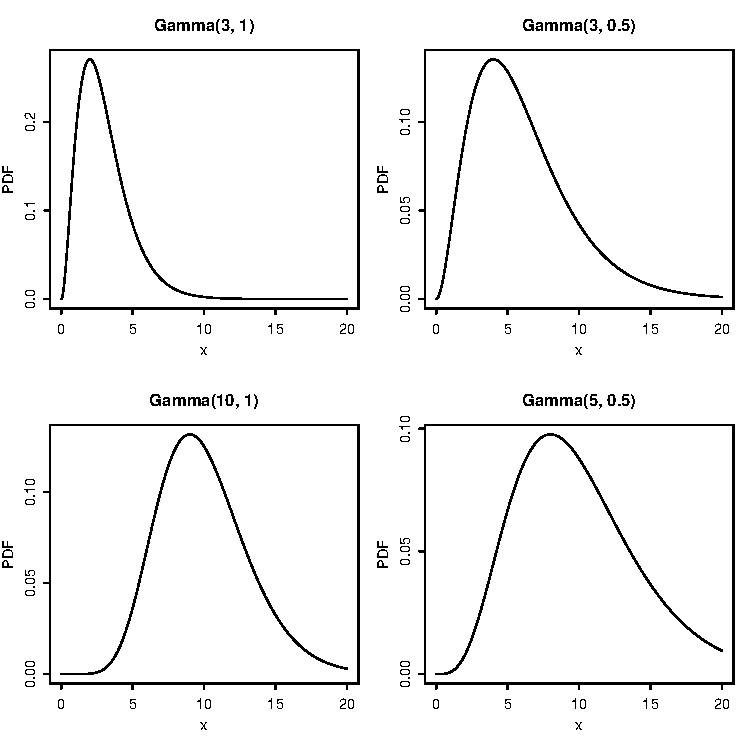
\includegraphics[width=1.9in]{figures/gammapdfs.pdf}
%%\end{minipage}
%%\medskip
%Let us say that $X$ is distributed $\Gam(a, \lambda)$. We know the following:
%\begin{description}
%	\item[Story] You sit waiting for shooting stars, where the waiting time for a star is distributed $\Expo(\lambda)$. You want to see $n$ shooting stars before you go home. The total waiting time for the $n$th shooting star is $\Gam(n,\lambda)$.
%	\item[Example]  You are at a bank, and there are 3 people ahead of you. The serving time for each person is Exponential with mean $2$ minutes. Only one person at a time can be served. The distribution of your waiting time until it's your turn to be served is $\Gam(3, \frac{1}{2})$.
%	%     \item[PDF] The PDF of a Gamma is:
%	% \begin{eqnarray*}
%	% f(x) = \frac{1}{\Gamma(a)}(\lambda x)^ae^{-\lambda x}\frac{1}{x},
%	% \hspace{.1 in}
%	% x \in [0, \infty)
%	% \end{eqnarray*}
%	% \item[Properties and Representations]
%	
%\end{description}
%
%\subsection{Beta Distribution}
%%\begin{minipage}{\linewidth}
%%	\centering
%%	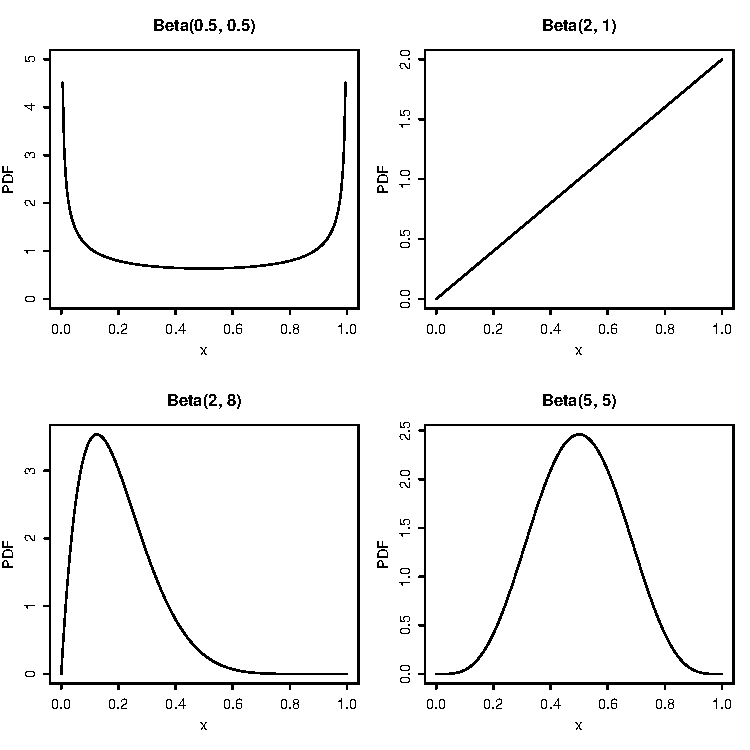
\includegraphics[width=1.9in]{figures/Betapdfs.pdf}
%%\end{minipage}
%%\medskip
%
%\begin{description}
%	
%	\item[Conjugate Prior of the Binomial] In the Bayesian approach to statistics, parameters are viewed as random variables, to reflect our uncertainty. The \emph{prior} for a parameter is its distribution before observing data. The \emph{posterior}  is the distribution for the parameter after observing data. Beta is the \emph{conjugate} prior of the Binomial because if you have a Beta-distributed prior on $p$ in a Binomial, then the posterior distribution on $p$ given the Binomial data is also Beta-distributed. Consider the following two-level model:
%	\begin{align*}
%	X|p &\sim \Bin(n, p) \\
%	p &\sim \Beta(a, b)
%	\end{align*}
%	Then after observing  $X = x$, we get the posterior distribution
%	\[p|(X=x) \sim \Beta(a + x, b + n - x) \]
%	
%	\item[Order statistics of the Uniform] See \emph{Order Statistics}.
%	\item[Beta-Gamma relationship] If $X \sim \Gam(a, \lambda)$, $Y \sim \Gam(b, \lambda)$, with $X \independent Y$ then
%	\begin{itemize}
%		\item $\frac{X}{X + Y} \sim \Beta(a, b)$
%		\item $X + Y \independent \frac{X}{X + Y}$
%	\end{itemize}
%	This is known as the \textbf{bank--post office result}.
%\end{description}
%
%
%% \[E(X) = \frac{a}{\lambda},  Var(X) = \frac{a}{\lambda^2}\]
%% \[X \sim G(a, \lambda),  Y \sim G(b, \lambda),  X \independent Y \rightarrow  X + Y \sim G(a + b, \lambda), \frac{X}{X + Y} \independent X + Y \]
%% \[X \sim \Gam(a, \lambda) \rightarrow X = X_1 + X_2 + ... + X_a \textnormal{ for $X_i$ i.i.d. $\Expo(\lambda)$} \]
%% \[\Gam(1, \lambda) \sim \Expo(\lambda) \]
%
%
%
%
%\subsection{Poisson Distribution} Let us say that $X$ is distributed $\Pois(\lambda)$. We know the following:
%\begin{description}
%	\item[Story] There are rare events (low probability events) that occur many different ways (high possibilities of occurences) at an average rate of $\lambda$ occurrences per unit space or time. The number of events that occur in that unit of space or time is $X$.
%	
%	\item[Example] A certain busy intersection has an average of 2 accidents per month. Since an accident is a low probability event that can happen many different ways, it is reasonable to model the number of accidents in a month at that intersection as $\Pois(2)$. Then the number of accidents that happen in two months at that intersection is distributed $\Pois(4)$.
%	
%	\item[Properties]
%	Let $X \sim \Pois(\lambda_1)$ and $Y \sim \Pois(\lambda_2)$, with $X \independent Y$.
%	
%	\begin{enumerate}
%		\itemsep -.5mm
%		\item \textbf{Sum} $X + Y \sim \Pois(\lambda_1 + \lambda_2)$
%		\item \textbf{Conditional} $X | (X + Y = n) \sim \Bin\left(n, \frac{\lambda_1}{\lambda_1 + \lambda_2}\right)$
%		\item \textbf{Chicken-egg} If there are $Z \sim \Pois(\lambda)$ items and we randomly and independently ``accept" each item with probability $p$, then the number of accepted items $Z_1 \sim \Pois(\lambda p)$, and the number of rejected items $Z_2 \sim \Pois(\lambda (1-p))$, and $Z_1 \independent Z_2$.
%	\end{enumerate}
%	
%	%     \item[PMF] The PMF of a Poisson is:
%	% \[P(X = k) = \frac{e^{-\lambda}\lambda^k}{k!}\]
%\end{description}
%
%\vspace*{2cm}
%
%
%	
%
%
%\vspace*{13cm}
%
%
%\section{Poisson Process}\smallskip \hrule height 2pt \smallskip
%
%\begin{description}
%\item[Definition] We have a \textbf{Poisson process} of rate $\lambda$ arrivals per unit time if the following conditions hold:
%\begin{enumerate}
%    \item The number of arrivals in a time interval of length $t$ is $\Pois(\lambda t)$.
%    \item Numbers of arrivals in disjoint time intervals are independent.
%\end{enumerate}
%For example, the numbers of arrivals in the time intervals $[0,5]$, $(5,12),$ and $[13,23)$ are independent with $\Pois(5\lambda), \Pois(7\lambda), \Pois(10\lambda)$ distributions, respectively.
%\begin{minipage}{\linewidth}
%            \centering
%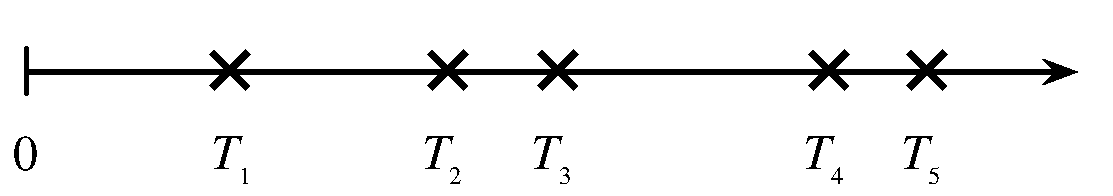
\includegraphics[width=2in]{figures/pp.pdf}
%        \end{minipage}
%       
%\item[Count-Time Duality]  Consider a Poisson process of emails arriving in an inbox at rate $\lambda$ emails per hour. Let $T_n$ be the time of arrival of the $n$th email (relative to some starting time $0$) and $N_t$ be the number of emails that arrive in $[0,t]$. Let's find the distribution of $T_1$. The event $T_1 > t$, the event that you have to wait more than $t$ hours to get the first email, is the same as the event $N_t = 0$, which is the event that there are no emails in the first $t$ hours. So
%\[P(T_1 > t) = P(N_t = 0) = e^{-\lambda t} \longrightarrow P(T_1 \leq t) = 1 - e^{-\lambda t}\]
%Thus we have $T_1 \sim \Expo(\lambda)$. By the memoryless property and similar reasoning, the interarrival times between emails are i.i.d.~$\Expo(\lambda)$, i.e., the differences $T_n - T_{n-1}$ are i.i.d.~$\Expo(\lambda)$.
%\end{description}
%
%\section{Order Statistics}\smallskip \hrule height 2pt \smallskip
%\begin{description}
%    \item[Definition] Let's say you have $n$ i.i.d.~r.v.s $X_1, X_2,\dots, X_n$. If you arrange them from smallest to largest, the $i$th element in that list is the $i$th order statistic, denoted $X_{(i)}$. So $X_{(1)}$ is the smallest in the list and $X_{(n)}$ is the largest in the list. \smallskip
%    
%     Note that the order statistics are \emph{dependent}, e.g., learning $X_{(4)} = 42$ gives us the information that $X_{(1)},X_{(2)},X_{(3)}$ are $\leq 42$ and $X_{(5)},X_{(6)},\dots,X_{(n)}$ are $\geq 42$.
%    \item[Distribution]  Taking $n$ i.i.d. random variables $X_1, X_2, \dots, X_n$ with CDF $F(x)$ and PDF $f(x)$, the CDF and PDF of $X_{(i)}$ are:
%        \[F_{X_{(i)}}(x) = P (X_{(i)} \leq x) = \sum_{k=i}^n {n \choose k} F(x)^k(1 - F(x))^{n - k}\]
%    \[f_{X_{(i)}}(x) = n{n - 1 \choose i - 1}F(x)^{i-1}(1 - F(x))^{n-i}f(x)\]
%%    \item[Universality of the Uniform] Let $X_1,X_2,\dots,X_n$ be i.i.d.~CRVs with CDF $F$, and let $U_j=F(X_j)$. By UoU, $U_1,U_2,\dots,U_n$ are i.i.d.~$\Unif(0,1)$. Since $F$ is increasing, $F(X_{(1)}) \leq F(X_{(2)}) \leq \dots \leq F(X_{(n)})$, so $U_{(j)} = F(X_{(j)})$.
%    \item[Uniform Order Statistics]  The $j$th order statistic of i.i.d.~$U_1,\dots,U_n \sim \Unif(0,1)$ is $U_{(j)} \sim \Beta(j, n - j + 1)$.
%\end{description}
%
%
%\section{Conditional Expectation}\smallskip \hrule height 2pt \smallskip
%\begin{description}
%    \item[Conditioning on an Event] We can find $E(Y|A)$, the expected value of $Y$ given that event $A$ occurred. A very important case is when $A$ is the event $X=x$. Note that $E(Y|A)$ is a \emph{number}. For example: 
%    \begin{itemize}
%    \item The expected value of a fair die roll, given that it is prime, is $\frac{1}{3} \cdot 2 + \frac{1}{3} \cdot 3 + \frac{1}{3} \cdot 5 = \frac{10}{3}$.
%    \item Let $Y$ be the number of successes in $10$ independent Bernoulli trials with probability $p$ of success. Let $A$ be the event that the first $3$ trials are all successes. Then
%    $$E(Y|A) = 3 + 7p$$
%    since the number of successes among the last $7$ trials is $\Bin(7,p)$. 
%        \item Let $T \sim \Expo(1/10)$ be how long you have to wait until the shuttle comes. Given that you have already waited $t$ minutes, the expected additional waiting time is 10 more minutes, by the memoryless property. That is, $E(T|T>t) = t + 10$.
%    \end{itemize}
%\end{description}
%        \scalebox{0.85}{
%                        \setlength{\extrarowheight}{7pt}
%            \begin{tabular}{ccc}
%                  \textbf{Discrete $Y$} & \textbf{Continuous $Y$} \\
%            \toprule
%            $E(Y) = \sum_y yP(Y=y)$ & $E(Y) =\int_{-\infty}^\infty yf_Y(y)dy$ \\
%           % $E(Y|X=x) = \sum_y yP(Y=y|X=x)$ & $E(Y|X=x) =\int_{-\infty}^\infty yf_{Y|X}(y|x)dy$ \\
%            $E(Y|A) = \sum_y yP(Y=y|A)$ & $E(Y|A) = \int_{-\infty}^\infty yf(y|A)dy$ \\ 
%            \bottomrule
%            \end{tabular}
%        }
%        \medskip
%\begin{description}
%    \item[Conditioning on a Random Variable]  We can also find $E(Y|X)$, the expected value of $Y$ given the random variable $X$. This is \emph{a function of the random variable $X$}. It is \emph{not} a number except in certain special cases such as if $X \independent Y$. To find $E(Y|X)$, find $E(Y|X = x)$ and then plug in $X$ for $x$. For example:
%    \begin{itemize}
%    \item If $E(Y|X=x) = x^3+5x$, then $E(Y|X) = X^3 + 5X$.
%    \item Let $Y$ be the number of successes in $10$ independent Bernoulli trials with probability $p$ of success and $X$ be the number of successes among the first $3$ trials. Then $E(Y|X)=X+7p$.
%    \item Let $X \sim \N(0,1)$ and $Y=X^2$. Then $E(Y|X=x) = x^2$ since if we know $X=x$ then we know $Y=x^2$. And $E(X|Y=y) = 0$ since if we know $Y=y$ then we know $X = \pm \sqrt{y}$, with equal probabilities (by symmetry). So $E(Y|X)=X^2, E(X|Y)=0$.  
%    \end{itemize} 
%    
%        \item[Properties of Conditional Expectation] \quad
%    \begin{enumerate}
%        \item $E(Y|X) = E(Y)$ if $X \independent Y$
%        \item $E(h(X)W|X) = h(X)E(W|X)$ (\textbf{taking out what's known}) \\
%        In particular, $E(h(X)|X) = h(X)$.
%        \item $E(E(Y|X)) = E(Y)$ (\textbf{Adam's Law}, a.k.a.~Law of Total Expectation)
%    \end{enumerate}
%
%    \item[Adam's Law (a.k.a.~Law of Total Expectation)]  can also be written in a way that looks analogous to LOTP. For any events $A_1, A_2, \dots, A_n$ that partition the sample space, 
%        \begin{align*}
%        E(Y) &= E(Y|A_1)P(A_1) + \dots + E(Y|A_n)P(A_n)
%    \end{align*}
%    For the special case where the partition is $A, A^c$, this says
%        \begin{align*}
%            E(Y) &= E(Y|A)P(A) + E(Y|A^c)P(A^c)
%    \end{align*}
%
%    \item[Eve's Law (a.k.a.~Law of Total Variance)] \quad
%    \[\var(Y) = E(\var(Y|X)) + \var(E(Y|X))\]
%\end{description}


\section{LLN \& CLT}\smallskip \hrule height 2pt \smallskip

\subsection{Law of Large Numbers (LLN)}
Let $X_1, X_2, X_3 \dots$ be i.i.d.~with mean $\mu$. The \textbf{sample mean} is $$\bar{X}_n = \frac{X_1 + X_2 + X_3 + \dots + X_n}{n}$$ The \textbf{Law of Large Numbers} states that as $n \to \infty$, $\bar{X}_n \to \mu$ with probability $1$. For example, in flips of a coin with probability $p$ of Heads, let $X_j$ be the indicator of the $j$th flip being Heads.  Then LLN says the proportion of Heads converges to $p$ (with probability $1$).

\subsection{Central Limit Theorem (CLT)}
%\subsubsection{Approximation using CLT}
%We use $\dot{\,\sim\,}$ to denote \emph{is approximately distributed}. We can use the \textbf{Central Limit Theorem} to approximate the distribution of a random variable $Y=X_1+X_2+\dots+X_n$ that is a sum of $n$ i.i.d. random variables $X_i$. Let  $E(Y) = \mu_Y$ and $\var(Y) = \sigma^2_Y$. The CLT says
%\[Y \dot{\,\sim\,} \N(\mu_Y, \sigma^2_Y)\]
%If the $X_i$ are i.i.d.~with mean $\mu_X$ and variance $\sigma^2_X$, then $\mu_Y = n \mu_X$ and $\sigma^2_Y = n \sigma^2_X$. For the sample mean $\bar{X}_n$, the CLT says
%\[ \bar{X}_n = \frac{1}{n}(X_1 + X_2 + \dots + X_n) \dot{\,\sim\,} \N(\mu_X, \sigma^2_X/n) \]


\subsubsection{Asymptotic Distributions using CLT}

We use $\xrightarrow{D}$ to denote \emph{converges in distribution to} as $n  \to \infty$. The CLT says that if we standardize the sum $X_1 + \dots + X_n$  then the distribution of the sum converges to $\N(0,1)$ as $n \to \infty$:
\[\frac{1}{\sigma\sqrt{n}} (X_1 + \dots + X_n - n\mu_X) \xrightarrow{D} \N(0, 1)\]
In other words, the CDF of the left-hand side goes to the standard Normal CDF, $\Phi$. In terms of the sample mean, the CLT says
\[ \frac{\sqrt{n} (\bar{X}_n - \mu_X)}{\sigma_X} \xrightarrow{D} \N(0, 1)\]

%\hrule height 2pt
%\section{\huge Metrics I} \hrule height 2pt
\section{Linear Algebra Review}
\hrule height 2pt
\subsection{Quadratic Forms}
	\smallskip
	A matrix $ \underset{q\times q}{A} $ is:
	\begin{itemize}
		\itemsep -.5mm
		\item \textbf{Positive Definite (p.d.)} if for any conformable vector $ \underset{q\times 1}{X} $, $ X'AX>0 $ for $ X\neq 0 $.
		\item \textbf{Positive Semi-Definite (p.s.d.)} if for any conformable vector $ \underset{q\times 1}{X} $, $ X'AX\geq0 $ for $ X\neq 0 $.
		\item \textbf{Negative Definite (n.d.)} if for any conformable vector $ \underset{q\times 1}{X} $, $ X'AX<0 $ for $ X\neq 0 $.
		\item \textbf{Negative Semi-Definite (n.s.d.)} if for any conformable vector $ \underset{q\times 1}{X} $, $ X'AX\leq0 $ for $ X\neq 0 $.
		\item \textbf{Indefinite} if $ X'AX<0 $ for some $ X $ and $ X'AX>0 $ for some other $ X $.
		\item $ \underset{(1\times q)}{X'}\underset{(q\times q)}{A}\underset{(q\times 1)}{X}=\sum_{i=1}^{q} \sum_{j=1}^{q} a_{ij}x_i x_j = a_{11} x_{1}^2 + a_{12}x_1 x_2 +a_{13} x_1 x_3 +...+a_{1q}x_1 x_q +a_{21}x_1 x_2+a_{22}x_2^2+...+a_{qq}x_q^2 $
		\item Any matrix of the from $ X'X $ is \textbf{positive semi-definite} (\textbf{p.s.d.}).
		\item If $ \underset{n\times k}{X} $ where $ \rho(X)=k $, that is, $ X $ has \textit{full column rank}, then $ X'X $ is p.d.
		\item If $ \underset{n\times k}{X},\ \rho(X)=k,\ \underset{n\times n}{D},\ d_{ij}>0 \forall i,\ \Rightarrow X'DX  $ is p.d. for diagonal matrix $ D $.
		\item If $ \underset{n\times k}{X},\ \rho(X)=k,\ \underset{n\times n}{D},\ d_{ij}>0 \forall i,\ \Rightarrow -X'DX  $ is n.d. for diagonal matrix $ D $.
	\end{itemize}
	\subsection{Derivatives}
		Let $ f(X) $ denote a \textit{scalar}-valued function where $ \underset{n\times 1}{X}\RA f:\Reals^n\to \Reals^1  $. Then we will define $ \frac{\partial \underset{1\times 1}{f(X)}}{ \partial \underset{n\times 1}{X}} = \begin{bmatrix}
		\frac{\partial f(X)}{\partial X_1} \\ \frac{\partial f(X)}{\partial X_1} \\ \vdots \\ \frac{\partial f(X)}{\partial X_n}
		\end{bmatrix} =\nabla f(X)$. \\ 
		Likewise $ \frac{\partial f(X)}{\partial X'}=\begin{bmatrix}
			\frac{\partial f(X)}{\partial X_1} \quad \frac{\partial f(X)}{\partial X_1} \quad \cdots \quad \frac{\partial f(X)}{\partial X_n}.
		\end{bmatrix} $

\end{multicols*}

\newpage 

\section{Table of Distributions}
%\begin{center}
%\renewcommand{\arraystretch}{3.9}
%\setlength{\aboverulesep}{1pt}
%\setlength{\belowrulesep}{1pt}
\begin{minipage}{.80\linewidth}
\resizebox{\textwidth}{!}{%
\begin{tabular}{ccccccc}
&\textbf{Distribution} & \textbf{PMF/PDF and Support} & CDF & \textbf{Expected Value}  & \textbf{Variance} & \textbf{MGF}\\
\toprule

\parbox[t]{2mm}{\multirow{15}{*}{\rotatebox[origin=c]{90}{\underline{\large Discrete}}}} 

&\shortstack{Bernoulli \\ \Bern($p$)} & \shortstack{$P(X=1) = p$ \\$ P(X=0) = q=1-p$} & $ F(x) =  \begin{cases} 0 & \text{if $ x<0 $} \\[-.5em] q & \text{if $ 0 \leq x < 1$} \\[-.5em] 1 & \text{if $ x \geq 1 $}  \end{cases} $ & $p$ & $pq$ & $q + pe^t$ \\
\cmidrule(l{2pt}r{2pt}){2-7}

&\shortstack{Binomial \\ \Bin($n, p$)} & \shortstack{$P(X=k) = {n \choose k}p^k q^{n-k}$  \\ $k \in \{0, 1, 2, \dots n\}$} & $ F(x) = \sum\limits_{i=0}^{\lfloor k \rfloor} {n \choose i} p^i q^{n-i} $ & $np$ & $npq$ & $(q + pe^t)^n$ \\
\cmidrule(l{2pt}r{2pt}){2-7}

&\shortstack{Geometric \\ \Geom($p$)} & \shortstack{$P(X=k) = q^kp$  \\ $k \in \{$0, 1, 2, \dots $\}$} & $ F(x) = 1-(1-p)^{k+1} $ & $q/p$ & $q/p^2$ & $\frac{p}{1-qe^t}, \, qe^t < 1$\\
\cmidrule(l{2pt}r{2pt}){2-7}

&\shortstack{Negative Binomial \\ \NBin($r, p$)} & \shortstack{$P(X=n) = {r + n - 1 \choose r -1}p^rq^n$ \\ $n \in \{$0, 1, 2, \dots $\}$} & Messy & $rq/p$ & $rq/p^2$ &  $(\frac{p}{1-qe^t})^r, \, qe^t < 1$\\
\cmidrule(l{2pt}r{2pt}){2-7}

&\shortstack{Hypergeometric \\ \Hypergeometric($w, b, n$)} & \shortstack{$P(X=k) = \sfrac{{w \choose k}{b \choose n-k}}{{w + b \choose n}}$ \\ $k \in \{0, 1, 2, \dots,  n\}$} & Messy & $\mu = \frac{nw}{b+w}$ &$\left(\frac{w+b-n}{w+b-1} \right) n\frac{\mu}{n}(1 - \frac{\mu}{n})$& Messy  \\
\cmidrule(l{2pt}r{2pt}){2-7}

&\shortstack{Poisson \\ \Pois($\lambda$)} & \shortstack{$P(X=k) = \frac{e^{-\lambda}\lambda^k}{k!}$ \\ $k \in \{$0, 1, 2, \dots $\}$} & Messy & $\lambda$ & $\lambda$ & $e^{\lambda(e^t-1)}$ \\
\cmidrule{1-7}

\parbox[t]{2mm}{\multirow{30}{*}{\rotatebox[origin=c]{90}{\underline{\large Continuous}}}} 

&\shortstack{Uniform \\ \Unif($a, b$)} & \shortstack{$ f(x) = \frac{1}{b-a}$ \\$ x \in (a, b) $} & $ F(x) =  \begin{cases} 0 & \text{if $ x<a $} \\[-.25em] \frac{x-a}{b-a} & \text{if $ a \leq x < b$} \\[-.25em] 1 & \text{if $ x \geq b $}  \end{cases} $ & $\frac{a+b}{2}$ & $\frac{(b-a)^2}{12}$ &  $\frac{e^{tb}-e^{ta}}{t(b-a)}$\\
\cmidrule(l{2pt}r{2pt}){2-7}

&\shortstack{Normal \\ $\N(\mu, \sigma^2)$} & \shortstack{$f(x) = \frac{1}{\sigma \sqrt{2\pi}} e^{-\sfrac{(x - \mu)^2}{(2 \sigma^2)}}$ \\ $x \in (-\infty, \infty)$} & Messy& $\mu$  & $\sigma^2$ & $e^{t\mu + \frac{\sigma^2t^2}{2}}$\\
\cmidrule(l{2pt}r{2pt}){2-7}

&\shortstack{Standard Normal \\ \\$\Phi(0, 1)$} & \shortstack{$\phi(x) = \frac{1}{ \sqrt{2\pi}} e^{-\sfrac{(x)^2}{(2 )}}$ \\ $x \in (-\infty, \infty)$} & Messy& $0$  & $1$ & $e^{ \frac{t^2}{2}}$\\
\cmidrule(l{2pt}r{2pt}){2-7}

&\shortstack{Log-Normal \\ $\mathcal{LN}(\mu,\sigma^2)$} & \shortstack{$\frac{1}{x\sigma \sqrt{2\pi}}e^{\sfrac{-(\log x - \mu)^2}{(2\sigma^2)}}$\\$x \in (0, \infty)$}& Messy & $ e^{ \mu + \sigma^2/2}$ & $ (e^{\sigma^2 + 2\mu})(e^{\sigma^2} - 1)$ & DNE \\
\cmidrule(l{2pt}r{2pt}){2-7}

&\shortstack{Exponential \\ $\Expo(\lambda)$} & \shortstack{$f(x) = \lambda e^{-\lambda x}$\\$ x \in (0, \infty)$} & $ F(x) = 1-e^{\lambda x} $ & $\frac{1}{\lambda}$  & $\frac{1}{\lambda^2}$ & $\frac{\lambda}{\lambda - t}, \, t < \lambda$\\
\cmidrule(l{2pt}r{2pt}){2-7}

&\shortstack{Erlang \\ $ \text{Erlang}_k(\lambda) $} & \shortstack{ $ f(x) = \frac{\lambda^k e^{-\lambda x} x^{k-1}}{(k-1)!},\  x\geq 0 $ \\ $ k= \{ 1,2,\hdots \},\ \lambda\in(0,\infty) $ } & $ F(x) = 1- \sum_{i=0}^{k-1} \frac{ e^{-\lambda x} (\lambda x)^i }{i!} $ & $ \frac{k}{\lambda} $ & $ \frac{k}{ \lambda ^2 } $ & $ \Big( \frac{\lambda}{\lambda - t}  \Big)^k   $ \\
\cmidrule(l{2pt}r{2pt}){2-7}

&\shortstack{Gamma \\ $\Gamma(\alpha, \beta)$} & \shortstack{$ f(x)= \left[ \frac{1}{\Gamma(\alpha) \beta^{\alpha} } \right] x^{\alpha-1} e^{-\frac{x}{\beta} }$ \\ $ x \in (0, \infty)$} & Messy& $ \alpha \beta $ & $ \alpha \beta^2 $ & $ (1-\beta t)^{-\alpha}, \, t < \beta$ \\
\cmidrule(l{2pt}r{2pt}){2-7}

&\shortstack{Beta \\  $ \mathcal{B}(\alpha, \beta) $} & \shortstack{$f(x) = \frac{\Gamma(\alpha+\beta)}{\Gamma(\alpha)\Gamma(\beta)}x^{\alpha-1}(1-x)^{\beta-1}$\\$x \in (0, 1) $} & Messy & $ \frac{\alpha}{\alpha + \beta}$  & $\frac{\alpha \beta}{(\alpha + \beta)^2(\alpha +\beta + 1)}$ & Messy \\
\cmidrule(l{2pt}r{2pt}){2-7}

&\shortstack{Chi-Square \\ $\chi_n^2$} & \shortstack{$\frac{1}{2^{n/2}\Gamma(n/2)}x^{n/2 - 1}e^{-x/2}$\\$x \in (0, \infty) $} & Messy & $n$  & $2n$ & $(1 - 2t)^{-n/2}, \, t < 1/2$\\
\cmidrule(l{2pt}r{2pt}){2-7}

&\shortstack{Student-$t$ \\ $t_n$} & \shortstack{$\frac{\Gamma((n+1)/2)}{\sqrt{n\pi} \Gamma(n/2)} (1+x^2/n)^{-(n+1)/2}$\\$x \in (-\infty, \infty)$} & Messy & $0$ if $n>1$ & $\frac{n}{n-2}$ if $n>2$ & DNE\\
\cmidrule(l{2pt}r{2pt}){2-7}

&\shortstack{F \\ $ \mathcal{F}(d_1,d_2) $} & \shortstack{$ f\left(x ; d_{1}, d_{2}\right)=\nicefrac{\left(\sqrt{\frac{\left(d_{1} x\right)^{d_{1}} d_{2}^{d_{2}}}{\left(d_{1} x+d_{2}\right)^{d_{1}+d_{2}}}}\right)}{x \mathcal{B}\left(\frac{d_{1}}{2}, \frac{d_{2}}{2}\right)} $\\$ x \in(0,+\infty) \text { if } d_{1}=1, \text { o/w } x \in[0,+\infty) $} & Messy & $ \frac{d_{2}}{d_{2}-2} $ & $ \frac{2 d_{2}^{2}\left(d_{1}+d_{2}-2\right)}{d_{1}\left(d_{2}-2\right)^{2}\left(d_{2}-4\right)} $ & DNE\\
\cmidrule(l{2pt}r{2pt}){2-7}

&\shortstack{Logistic \\ $\sec^2$} & \shortstack{$ \psi(x)=\frac{e^x}{1+e^x}\left[ 1-\frac{e^x}{1+e^x} \right] $\\$x \in (-\infty, \infty)$} & $ \Psi(x)= \frac{e^x}{1+e^x} $ & 0 & $\frac{\pi^2}{3} $ & \shortstack{ $ e^t *\mathcal{B}(1-t,1+t) $ \\ for $ t\in(-1,1) $}\\

\bottomrule
\end{tabular}

}

\end{minipage}
%
%
%\begin{multicols*}{4}
%	\tiny
%	
%	% multicol parameters
%	% These lengths are set only within the two main columns
%	%\setlength{\columnseprule}{0.25pt}
%	\setlength{\premulticols}{1pt}
%	\setlength{\postmulticols}{1pt}
%	\setlength{\multicolsep}{1pt}
%	\setlength{\columnsep}{2pt}
%	\setlength{\abovedisplayskip}{0pt}
%	\setlength{\belowdisplayskip}{0pt}
%
%\textbf{\textcolor{FSGarnet}{Intersections via Conditioning}}
%\begin{align*} 
%P(A\cap B) &= P(A)P(B|A) \\
%P(A\cap B\cap C) &= P(A)P(B|A)P(C|A\cap B) 
%\end{align*}
%
%
%\textbf{\textcolor{FSGarnet}{Expected value of a function of an r.v.}}
%The expected value of $X$ is defined this way:
%\[E(X) = \sum_x xP(X=x) \textnormal{ (for discrete $X$)}\]
%\[E(X) = \int^\infty_{-\infty}xf(x)dx  \textnormal{ (for continuous $X$)}\]
%You can find the expected value of a \emph{function of a random variable}, $h(X)$, by replacing the $x$ in front of the PMF/PDF by $h(x)$ but still working with the PMF/PDF of $X$:
%\[E(h(X)) = \sum_x h(x)P(X=x) \textnormal{ (for discrete $X$)}\]
%\[E(h(X)) = \int^\infty_{-\infty}h(x)f(x)dx \textnormal{ (for continuous $X$)}\]
%Expected value is \emph{linear}. This means that for \emph{any} random variables $X$ and $Y$ and any constants $a, b, c$, the following is true:
%\[E(aX + bY + c) = aE(X) + bE(Y) + c\]
%
%
%
%\textbf{\textcolor{FSGarnet}{Moments}}\\
%Let $X$ have mean $\mu$ and standard deviation $\sigma$, then: \\
%
%The $ k^{th}$ \textbf{moment} of a RV, $ X $, is $ E[X^k] = \SumInt x^k f(x) $.\\
%The $ k^{th}$ \textbf{central moment} of a RV, $ X $, is $ E[(X-\mu)^k] = \SumInt (x-\mu)^k f(x) $.
%
%The mean and variance are important summaries of the shape of a distribution.
%\begin{description}
%	\item[Mean] $E(X) = \mu_1 $
%	\item[Variance] $\var(X) = \mu_2 - \mu_1^2$
%	%        \item[Skewness] $\textrm{Skew}(X) = m_3$
%	%      \item[Kurtosis] $\textrm{Kurt}(X) = m_4 - 3$
%\end{description}
%
%\textbf{\textcolor{FSGarnet}{Moment Generating Functions:}}
%\begin{description}
%	\item[MGF] For any random variable $X$, the function
%	\[ M_X(t) = E(e^{tX}) \]
%	is the \textbf{moment generating function (MGF)} of $X$, if it exists for all $t$ in some open interval containing $0$.
%	
%	\item[Why is it called the Moment Generating Function?] Because the $k$th derivative of the moment generating function, evaluated at $0$, is the $k$th moment of $X$.
%	\[\mu_k = E(X^k) = M_X^{(k)}(0)\]
%%	This is true by Taylor expansion of $e^{tX}$ since
%%	\[M_X(t) = E(e^{tX}) = \sum_{k=0}^\infty \frac{E(X^k)t^k}{k!} = \sum_{k=0}^\infty \frac{\mu_k t^k}{k!} \]
%	\item[MGF of linear functions] If we have $Y = aX + b$, then
%	\[M_Y(t) = E(e^{t(aX + b)}) =  e^{bt}E(e^{(at)X}) = e^{bt}M_X(at)\]
%	\item[Uniqueness] \emph{If it exists, the MGF uniquely determines the distribution}. This means that for any two random variables $X$ and $Y$, they are distributed the same (their PMFs/PDFs are equal) if and only if their MGFs are equal. 
%	\item[Summing Independent RVs by Multiplying MGFs.] If $X$ and $Y$ are independent, then
%	\begin{align*}
%	M_{X+Y}(t) &= E(e^{t(X + Y)}) = E(e^{tX})E(e^{tY}) = M_X(t) \cdot M_Y(t) 
%	\end{align*}
%	The MGF of the sum of two random variables is the product of the MGFs of those two random variables.
%\end{description}
%
%
%
%\textbf{\textcolor{FSGarnet}{Joint Distributions}}
%The \textbf{joint CDF} of $X$ and $Y$ is 
%$$F(x,y)=P(X \leq x, Y \leq y)$$
%In the discrete case, $X$ and $Y$ have a \textbf{joint PMF} 
%$$p_{X,Y}(x,y) = P(X=x,Y=y).$$ In the continuous case, they have a \textbf{joint PDF}
%\[f_{X,Y}(x,y) = \frac{\partial^2}{\partial x \partial y} F_{X,Y}(x,y).\]
%The joint PMF/PDF must be nonnegative and sum/integrate to 1.\\
%%\begin{minipage}{\linewidth}
%%            \centering
%%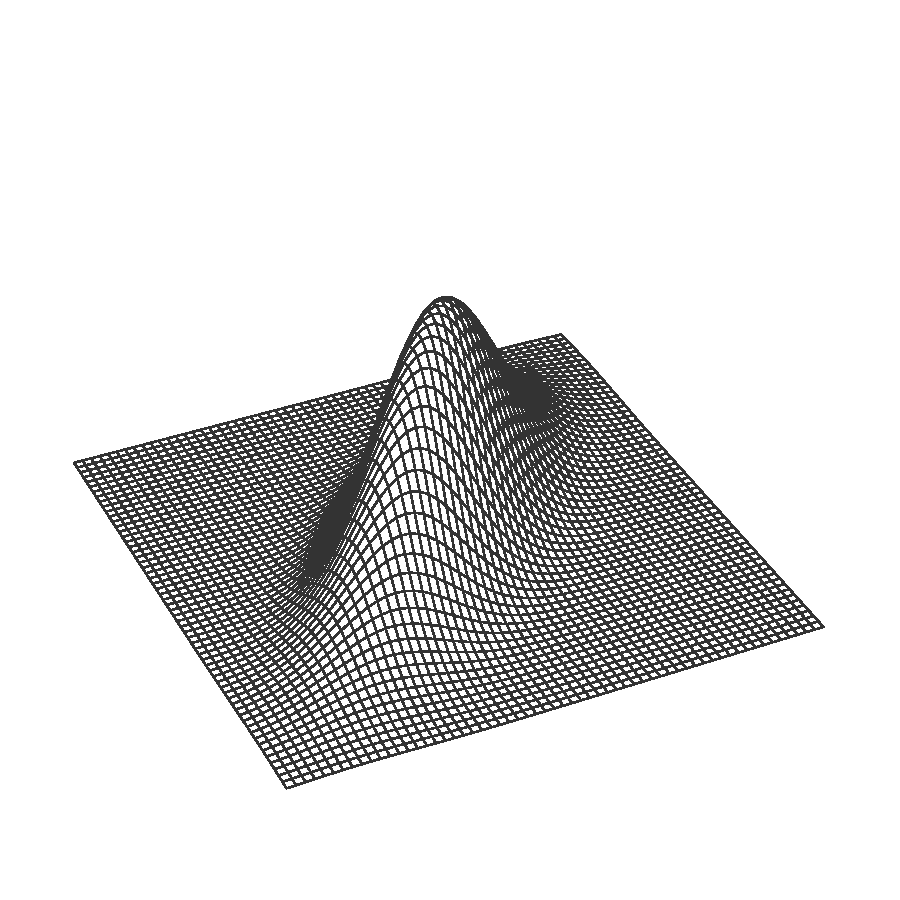
\includegraphics[width=1.0in]{figures/jointPDF.pdf}
%%        \end{minipage}
%
%\textbf{\textcolor{FSGarnet}{Marginal Distributions}}
%To find the distribution of one (or more) random variables from a joint PMF/PDF, sum/integrate over the unwanted random variables. \medskip
%
%\textbf{Marginal PMF from joint PMF}
%\[P(X = x) = \sum_y P(X=x, Y=y)\]
%\textbf{Marginal PDF from joint PDF}
%\[f_X(x) = \int_{-\infty}^\infty f_{X, Y}(x, y) dy\]
%
%\textbf{Limits of marginals and expected values:} Note that the only time you are integrating over \textit{all} the possible values of $ Y $ for the continuous case is when you are trying to find its expected value. \\
%For example, given iid RV's $ X,Y$, w/ pdf $ f(x,y)=3x,\ 0<y<x<1 $
%
%$ \Rightarrow E[X] = \int_{- \infty}^{\infty} xf_X (x) dx = \int_{- \infty}^{\infty} x[ \int_{- \infty}^{\infty } f(x,y) dy ] dx =  \int_{- \infty}^{\infty}x [ \int_{0}^{x} 3x dy ] dx =  \int_{- \infty}^{\infty} x [ 3x^2,\ 0<x<1 ] dx = \int_{0}^{1} x3x^2 dx = \frac{3}{4} $  
%
%However note that $ E[XY] = \int_{-\infty}^{\infty} \int_{-\infty}^{\infty} xy\ f(x,y)\ dy\ dx $, which using the previous joint pdf: $ = \int_{0}^{1} \int_{0}^{x} xy\ 3x\ dy\ dx $ \\
%
%\textbf{\textcolor{FSGarnet}{Conditional Distributions}}\\
%\textbf{Conditioning for discrete r.v.s}
%\[P(Y=y|X=x) = \frac{P(X=x, Y=y)}{P(X=x)} \]
%\textbf{Conditioning for continuous r.v.s}
%\[f_{Y|X}(y|x) = \frac{f_{X,Y}(x, y)}{f_X(x)} \]
%%\textbf{Hybrid Bayes' rule}
%%\[f_X(x|A) = \frac{P(A | X = x)f_X(x)}{P(A)}\]
%
%
%\textbf{\textcolor{FSGarnet}{Conditional Expectations}}
%\scalebox{0.85}{
%	\setlength{\extrarowheight}{7pt}
%	\begin{tabular}{ccc}
%		\textbf{Discrete $X$} & \textbf{Continuous $X$} \\
%		\toprule
%		$E(X) = \sum_x xP(X=x)$ & $E(X) =\int_{-\infty}^\infty xf_X(x)dx$ \\
%		% $E(Y|X=x) = \sum_y yP(Y=y|X=x)$ & $E(Y|X=x) =\int_{-\infty}^\infty yf_{Y|X}(y|x)dy$ \\
%		$E(X|A) = \sum_x xP(X=x|A)$ & $E(X|A) = \int_{-\infty}^\infty xf(x|A)dx$ \\ 
%		\bottomrule
%	\end{tabular}
%}
%
%	\textbf{Conditioning on a Random Variable}  We can also find $E(Y|X)$, the expected value of $Y$ given the random variable $X$. This is \emph{a function of the random variable $X$}. It is \emph{not} a number except in certain special cases such as if $X \independent Y$. To find $E(Y|X)$, find $E(Y|X = x)$ and then plug in $X$ for $x$. For example:
%	\begin{itemize}
%		\itemsep -.5mm
%		\item If $E(Y|X=x) = x^3+5x$, then $E(Y|X) = X^3 + 5X$.
%		\item Let $Y$ be the number of successes in $10$ independent Bernoulli trials with probability $p$ of success and $X$ be the number of successes among the first $3$ trials. Then $E(Y|X)=X+7p$.
%		\item Let $X \sim \N(0,1)$ and $Y=X^2$. Then $E(Y|X=x) = x^2$ since if we know $X=x$ then we know $Y=x^2$. And $E(X|Y=y) = 0$ since if we know $Y=y$ then we know $X = \pm \sqrt{y}$, with equal probabilities (by symmetry). So $E(Y|X)=X^2, E(X|Y)=0$.  
%	\end{itemize} 
%	
%	\textbf{Properties of Conditional Expectation}
%	\begin{enumerate}
%		\item $E(Y|X) = E(Y)$ if $X \independent Y$
%		\item $E(h(X)W|X) = h(X)E(W|X)$ (\textbf{taking out what's known}) \\
%		In particular, $E(h(X)|X) = h(X)$.
%		\item $E(E(Y|X)) = E(Y)$ (\textbf{Law of Iterated Expectation})
%	\end{enumerate}
%
%\textbf{\textcolor{FSGarnet}{One Variable Transformations}} Let's say that we have a random variable $X$ with PDF $f_X(x)$, but we are also interested in some function of $X$. We call this function $Y = g(X)$. Also let $y=g(x)$. If $g$ is differentiable and strictly increasing (or strictly decreasing), then the PDF of $Y$ is
%\[f_Y(y) = f_X(x)\left|\frac{dx}{dy}\right| =  f_X(g^{-1}(y))\left|\frac{d}{dy}g^{-1}(y)\right|\]
%The derivative of the inverse transformation is called the \textbf{Jacobian}.\\
%
%
%
%\end{multicols*}
%

%\end{center}


\end{document}
